\section{Analysis Strategy}
\label{sec:AnalysisStrategy}
We take different analysis approaches between the below and above 3 TeV signal mass samples. In the analyses below 3 TeV, we adopt the multivariable analyses by training boosted decision tree (BDT) on every mass point. On the other hand, for the mass points above 3 TeV, we adopt the cut-and-counting approach. We describe these strategies below.

\subsection{Analysis strategy below 3 TeV}
\label{subsec:AnaStrategyUnder3TeV}
\subsubsection{Event Selection}
\label{subsubsec:RegionDefUnder3TeV}
In the analysis below 3 TeV signal mass points, two signal regions, ``SR1'' and ``SR2'', are defined according to the numbers of leptons, top tagged large-$R$ jets, and $b$-tagged small-$R$ jets. 

Figure \ref{fig:EventTopology_Htb} shows the schematic of boosted event topology of an $H^{+}{\rightarrow}tb$ event. A signal event is expected to have one $J_{\text{top-tag}}$, three $b$-jets, and one lepton+MET. However, the $b$-jet originated from the gluon is typically not detectable because it tends to fly in the forward directions and outside the detector acceptance. Therefore, at least two $b$-jets are required in this analysis.

Events in the inclusive signal region (SR) are required to have exactly one lepton ($e$ or ${\mu}$) that is matched to the one firing one of the single lepton triggers to be consistent with the signal event, as shown in Figure \ref{fig:EventTopology_Htb}. Events must also have at least one top-tagged large-$R$ jet, at least two small-$R$ jets, and at least two $b$-tagged small-$R$ jets. These small-$R$ jets must additionally satisfy ${\Delta}R(J_{\text{top-tag}}^{1\text{st}}, jet)>1.0$ to ensure these small-$R$ jets are not constituent of the leading top-tagged jet. This analysis does not require missing $E_{T}$. 

Events are further split into SR1 and SR2 depending on the number of b-tagged small-R jets. Those having exactly two (at least three) b-tagged small-R jets are categorized into SR1 (SR2). As shown in Figure \ref{fig:BkgComposition_SR1}, SR1 is enriched in $t\Bar{t}+\text{light}$ events, while SR2 is enriched in $t\Bar{t}+\text{heavy flavor (HF)}$ events. These features can be used to constrain each background in the fit.

%--- Figure of Event Topology
\begin{figure}[H]
  \centering
  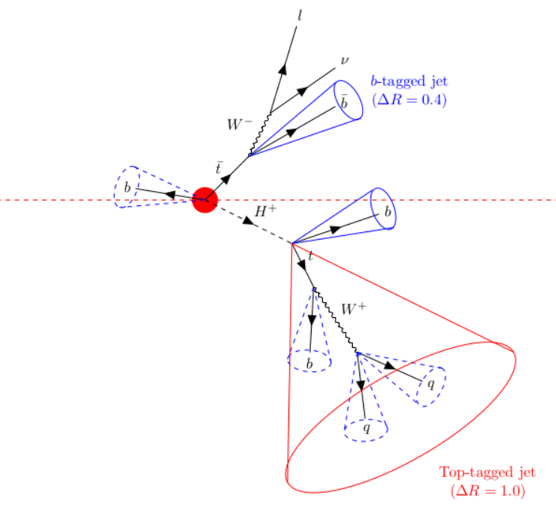
\includegraphics[keepaspectratio,scale=0.8]{images/AnalysisStrategy/EventTopology.png}
  \caption{Schematic of boosted event topology. Signal event has one $J_{\text{top-tag}}$ and at least two $b$-tagged small-$R$ jets.}
  \label{fig:EventTopology_Htb}
\end{figure}
%---

%--- Table of SR1 Event Selections
\begin{table}[H]
  \centering
  \begin{tabular*}{170mm}{l|ll|l}
    \hline\hline
    Cut                       & SR1                                                         &                           & SR2\\
    \hline
    leptons                   &  - $\text{N}_{\text{lepton}}=1$                             &                           & \\
                              & \underline{Electron}                                        & \underline{Muon}          & Same as SR1\\
                              &  - $p_{\text{T}}>27$ GeV                                    &  - $p_{\text{T}}>27$ GeV  & \\
                              &  - $|\eta|<1.37$ or $1.52<|\eta|<2.47$                      &  - $|\eta|<2.5$           & \\
    \hline
    Top-tagged large-$R$ jets &  - $\text{N}_{J_{\text{top-tag}}} \geq 1$                   &                           &\\
                              &  - $350~\text{GeV}<p_{\text{T}}<2500~\text{GeV}$            &                           & Same as SR1\\
                              &  - $m>40\text{GeV}$                                         &                           & \\
    \hline
    Small-$R$ jets            &  - $\text{N}_{\text{jet}} \geq 2$                           &                           & $\text{N}_{\text{jet}} \geq 3$ \\
                              &  - $p_{\text{T}}>25$ GeV                                    &                           & (Kinematic requirements\\
                              &  - $|\eta|<2.5$                                             &                           &  are same as SR1)\\
                              &  - ${\Delta}R(J_{\text{top-tag}}^{1st}, jet)>1.0$           &                           & \\
    \hline
    $b$-tagged small-$R$ jets & $\text{N}_{b-\text{jet}} = 2$                               &                           & $\text{N}_{b-\text{jet}} \geq 3$\\

    \hline\hline
  \end{tabular*}
  \caption{Event selections in the SR1 and SR2. After these selections, SR1 becomes enriched in $t\bar{t}+\text{light}$, and SR2 becomes enriched in $t\bar{t}+\text{HF}$}
  \label{tab:EventSelectionInSR1AndSR2}
\end{table}

%--- Figure for SR1
\begin{figure}[H]
  \centering
  \subfloat[]{
    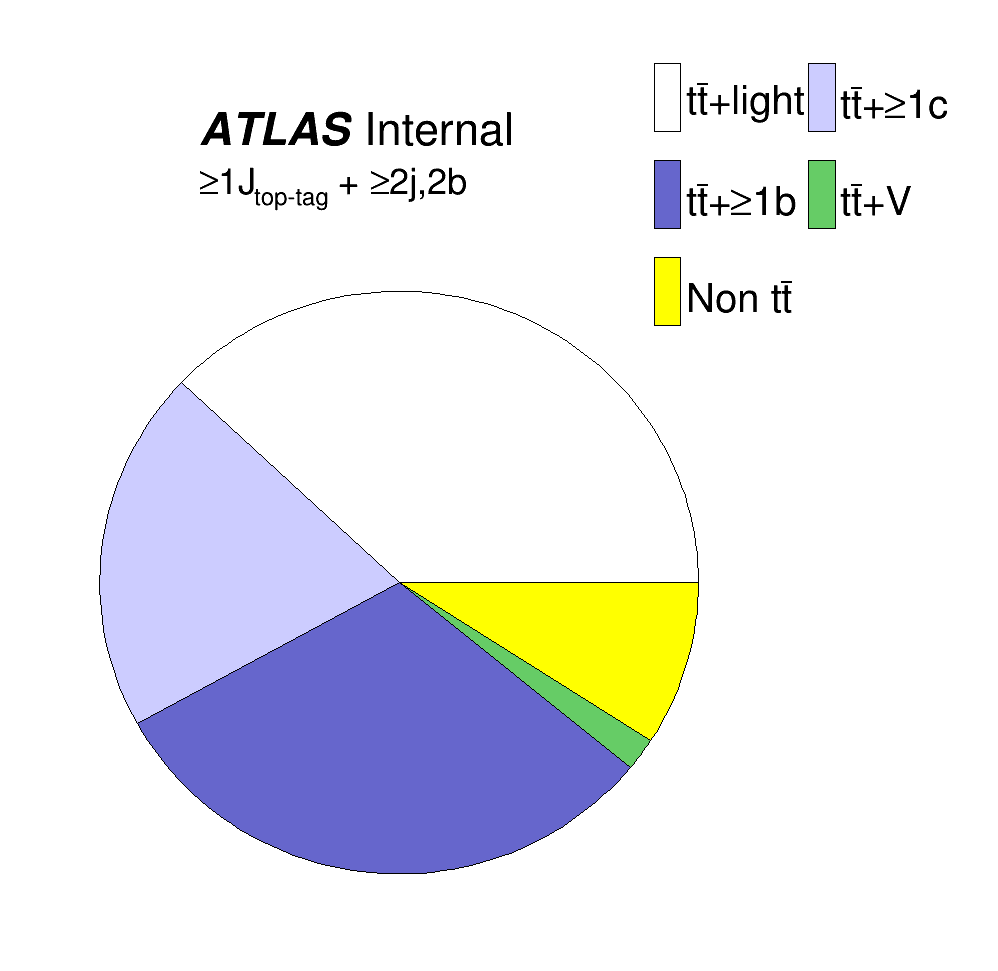
\includegraphics[keepaspectratio,scale=0.2]{images/AnalysisStrategy/PieChart_SR1.png}
    \label{fig:PieChart_SR}
  }
  \subfloat[]{
    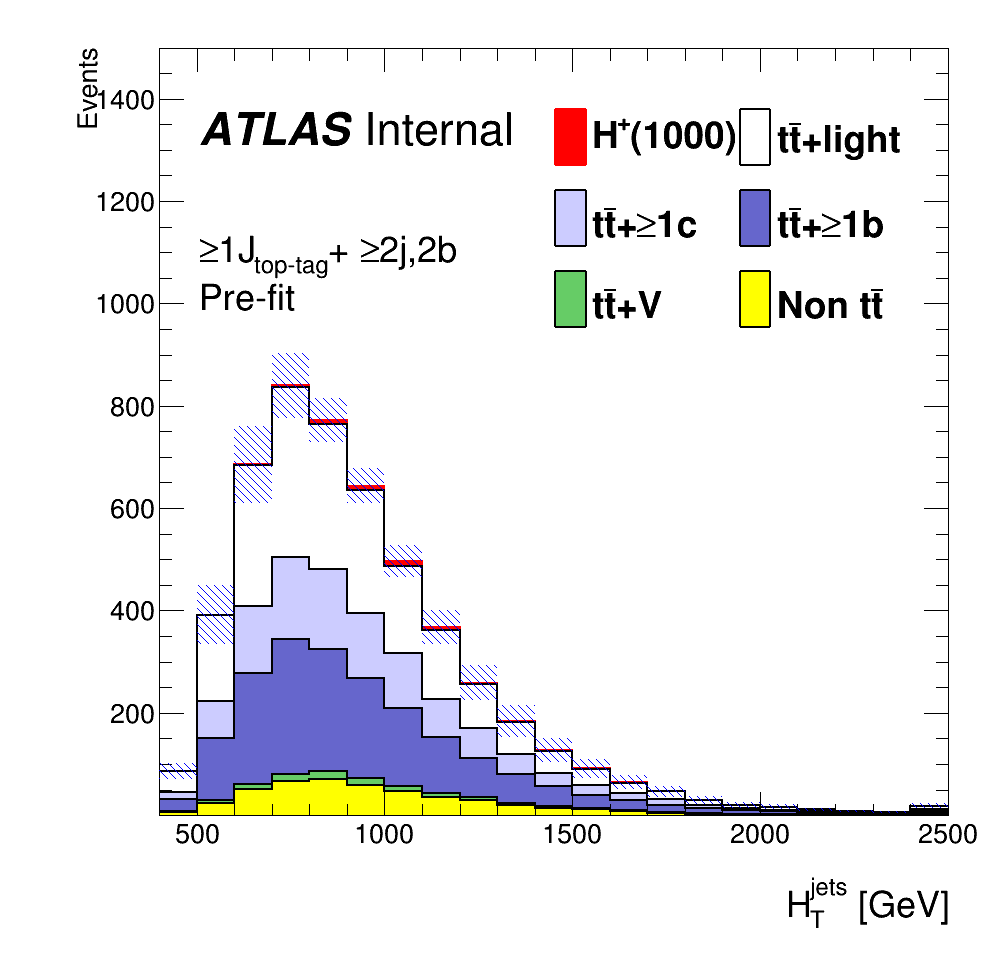
\includegraphics[keepaspectratio,scale=0.2]{images/AnalysisStrategy/HT_jets_SR1.png}
    \label{fig:PieChart_SR1}
  }
  \caption{Background composition in the SR1 is shown in the pie chart (a) and the $H_{\text{T}}^{\text{jets}}$ distributions (b).}
  \label{fig:BkgComposition_SR1}
\end{figure}


%--- Figure for SR2
\begin{figure}[H]
  \centering
  \subfloat[]{
    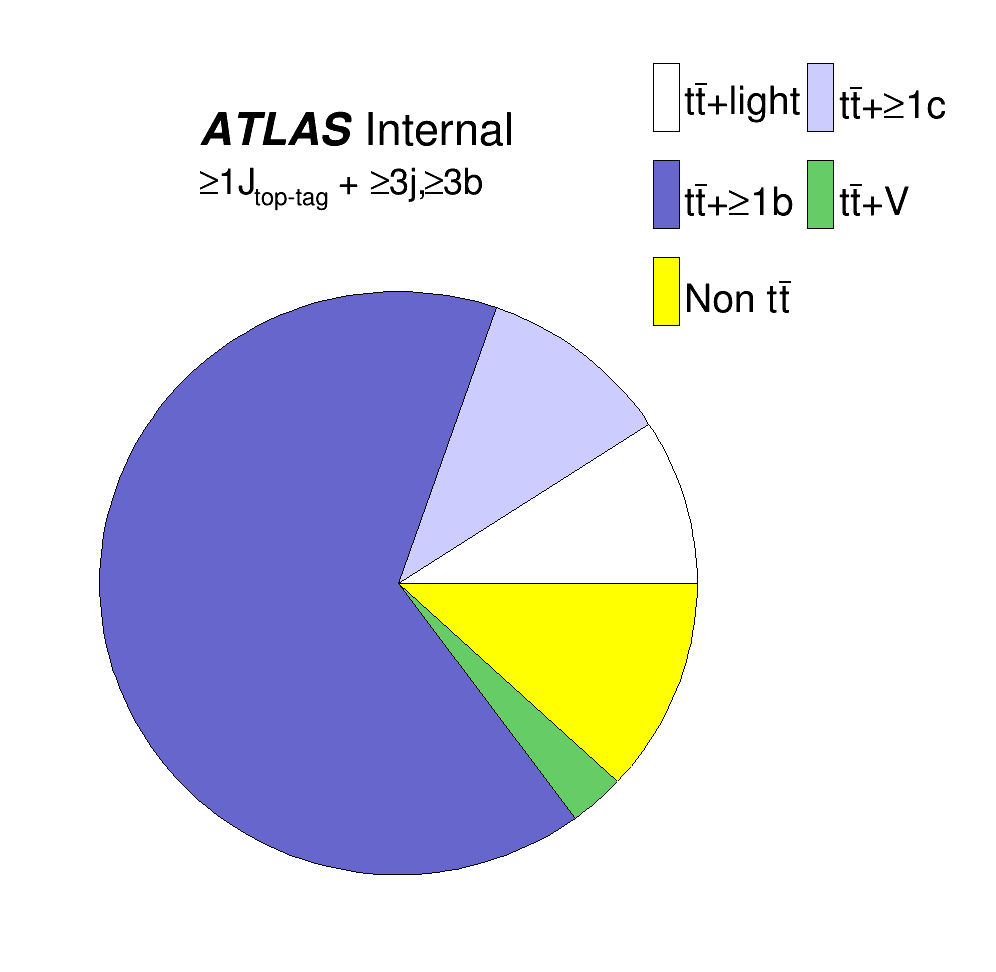
\includegraphics[keepaspectratio,scale=0.2]{images/AnalysisStrategy/PieChart_SR2.png}
    \label{fig:PieChart_SR}
  }
  \subfloat[]{
    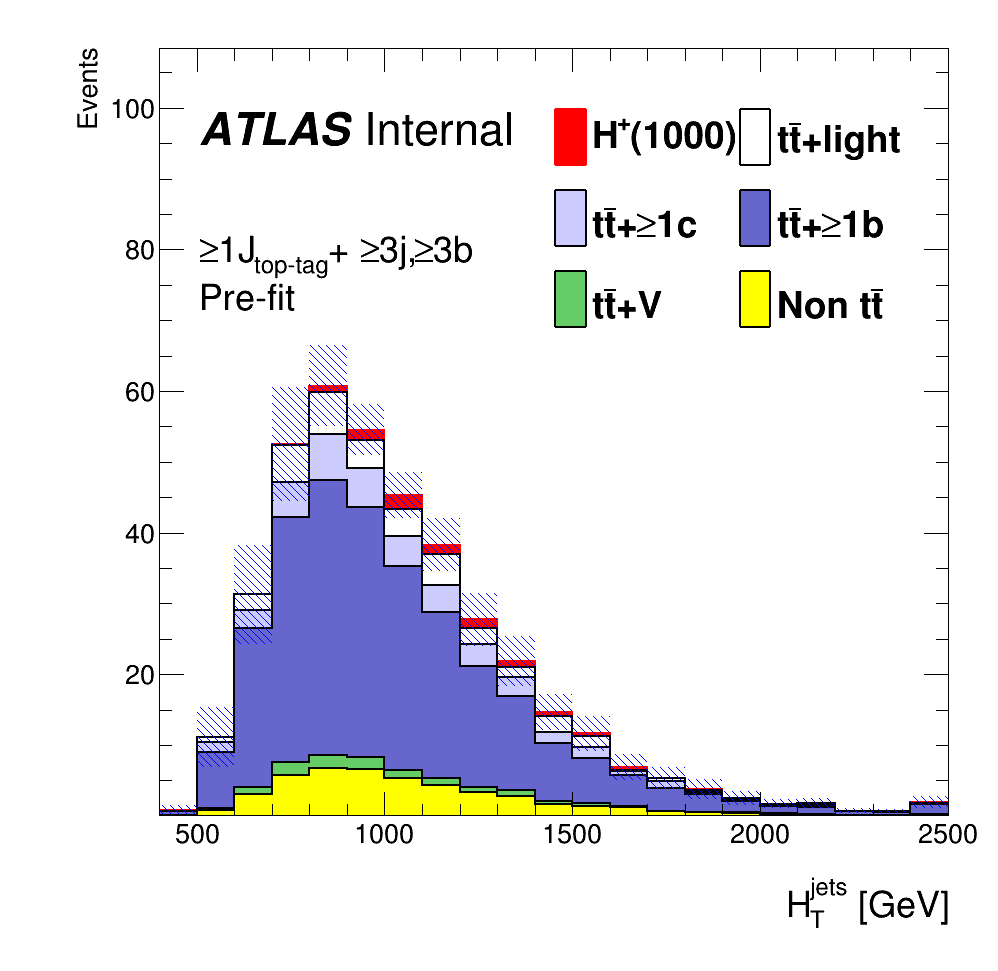
\includegraphics[keepaspectratio,scale=0.2]{images/AnalysisStrategy/HT_jets_SR2.png}
    \label{fig:PieChart_SR1}
  }
  \caption{Background composition in the SR2 is shown in the pie chart (a) and the $H_{\text{T}}^{\text{jets}}$ distributions (b).}
  \label{fig:BkgComposition_SR2}
\end{figure}

The expected number of signal and background events in the SR1 and SR2 are shown in Table \ref{tab:PrefitYields}. For the predicted number of $H^{+}$ signal events with the 1000 and 3000 GeV mass hypothesis, the cross-section of ${\sigma}(pp{\rightarrow}tbH^{+}){\times}Br(H^{+}{\rightarrow}tb)=0.046$ pb is assumed. This corresponds to the upper limit at $M_{H^{+}}=1000$ GeV obtained from the resolved analysis \cite{HDBS-2021-02}. As discussed later in Section \ref{subsec:BlindStrategy}, we use the signal ${\sigma}{\times}Br$ to define the blinded regions.

\begin{table}[H]
  \centering
  \begin{tabular*}{120mm}{@{\extracolsep{\fill}}cll}
    \hline\hline
                            & \multicolumn{1}{c}{SR1} & \multicolumn{1}{c}{SR2}\\
    \hline
    $t\bar{t}+\text{light}$ & $1943\pm 87$           & $   35\pm  4$ \\
    $t\bar{t}+\geq1c$       & $1029\pm 54$           & $   41\pm  5$ \\
    $t\bar{t}+\geq1b$       & $1588\pm 69$           & $  253\pm 15$ \\
    $t\bar{t}+W$            & $  36\pm 19$           & $   52\pm 27$ \\
    $t\bar{t}+Z$            & $  57\pm  9$           & $    2\pm  1$ \\
    $Wt$ channel            & $ 176\pm 89$           & $    9\pm  2$ \\
    $t$ channel             & $  36\pm  3$           & $    1\pm  0$ \\
    Other top sources       & $  30\pm 11$           & $    9\pm  4$ \\
    $VV$, $V$+jets          & $ 147\pm 53$           & $    5\pm  2$ \\
    $t\bar{t}H$             & $  79\pm  3$           & $   24\pm  1$ \\
    \hline
    Total                   & $5120\pm230$           & $  387\pm 24$ \\
    \hline
    $H^{+}$ 1000 GeV        & $  46\pm  5$           & $    9\pm  2$ \\
    $H^{+}$ 3000 GeV        & $  60\pm 14$           & $   13\pm  3$ \\
    \hline\hline
  \end{tabular*}
  \caption{Number of expected events in each analysis region. The quoted uncertainties include both statistical and systematic uncertainties before fitting.}
  \label{tab:PrefitYields}
\end{table}

\subsubsection{Multivariable analysis using BDT}
\label{subsec:MVA}

In this search, the most important background is $t\bar{t}+\text{jets}$ as discussed in Section \ref{subsec:AnaStrategyUnder3TeV}. To enhance the separation between signal and background, multivariable analysis is performed using Boosted Decision Trees (BDT) technique of TMVA \cite{TMVA}. Obtained BDT score distribution is used in the profile likelihood fit as a final discriminant (Section \ref{sec:ProfileLikelohoodFit}).

\begin{description}
    \item{\textbf{Signal and background definition in BDT training}}\mbox{}\\
    To classify signal ($H^{+}$ and $W'$) and $t\bar{t}+\text{jets}$ background events, BDTs are trained using the simulated $H^{+}$ signal and $t\bar{t}+\text{jets}$ background samples. This analysis under 3 TeV mass points considers eight different mass hypotheses, and the training is performed on each mass hypothesis. On the other hand, the $t\bar{t}+\text{jets}$ background samples are common in each training. Since kinematics of $H^+$ signals become harder in higher mass hypotheses, the BDTs trained using the higher $H^{+}$ mass samples typically have greater separation power. These signal events and background events used in training are required to pass either SR1 or SR2 criteria. These BDTs optimized using $H^{+}$ signal samples can be also used in $W' \rightarrow tb$ analysis because the difference between a $H^{+}$ and $W'$ is only their spin and the kinematic characteristics of $W' \rightarrow tb$ events are similar to the ones of $H^{+} \rightarrow tb$ events. This validation is done in the section below. BDTs are also trained using 4 and 5 TeV mass point samples. These BDT outputs are only used for the study in Section \ref{subsec:ReweightingTechnique}.

    \item{\textbf{BDT training settings}}\mbox{}\\
    To fully use the simulation samples' statistics, we adopt the 4-fold cross-validation method in the BDT training (Figure \ref{fig:CrossValidationScheme}). Each simulation sample is divided into four sub-datasets (Fold1, Fold2, Fold3, and Fold4). For each MC event, a random number is generated with the MC event number as a seed, and the event is categorized into one of the sub-datasets according to the generated number. Two of the four sub-datasets are labeled "TRAIN," which are used for BDT training. One of the other sub-datasets is labeled "VALID" and is used to optimize the BDT performance. The last sample, "TEST" is used to construct a fit template. Four combinations of sub-dataset usage (Split1 to Split4 in Figure \ref{fig:CrossValidationScheme}) are tried, and we obtain four statistically-independent BDTs and fit templates. They are combined into one fit template used in the profile likelihood fit (Section.\ref{sec:ProfileLikelohoodFit}).
    
    \begin{figure}[H]
        \centering
        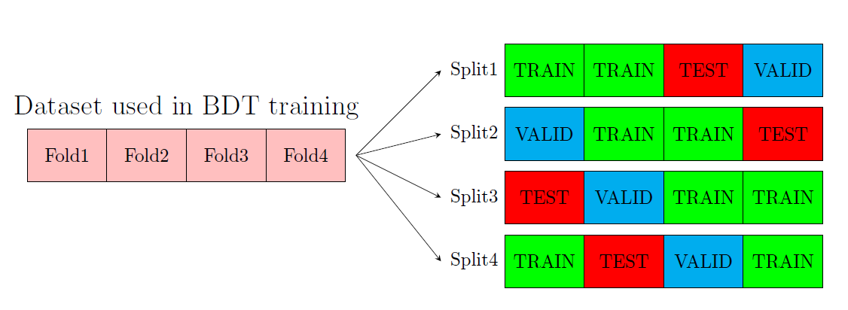
\includegraphics[keepaspectratio,scale=0.65]{images/AnalysisStrategy/CrossValidationScheme.png}
        \caption{Scheme of 4-fold cross-validation of BDT in this analysis.}
        \label{fig:CrossValidationScheme}
    \end{figure}
    
    Hyperparameters for the BDTs are summarized in Table. \ref{tab:Hyperparameters}. Those hyperparameters are chosen to obtain the best sensitivity.

    \begin{table}[H]
      \centering
      \begin{tabular*}{75mm}{@{\extracolsep{\fill}}ll}
        \hline
        \multicolumn{1}{c}{Configuration} & \multicolumn{1}{c}{}\\
        \hline\hline
        \multicolumn{1}{l}{Algorithm}     & \multicolumn{1}{c}{Gradient boosting}\\
        \hline
        $Hyperparameters$ & \\
        \multicolumn{1}{l}{NTrees}       & \multicolumn{1}{c}{100}\\
        \multicolumn{1}{l}{MinNodeSize}  & \multicolumn{1}{c}{2.5}\\
        \multicolumn{1}{l}{MaxDepth}     & \multicolumn{1}{c}{3}\\
        \multicolumn{1}{l}{nCuts}        & \multicolumn{1}{c}{20}\\
        \hline
      \end{tabular*}
      \caption{List of hyperparameters used in the training of a BDT}
      \label{tab:Hyperparameters}
    \end{table}

    \item{\textbf{Input variables in BDT}}\mbox{}\\
    \label{item:BDTInputVars}
    Jets originating from a $H^{+}$ ($W'$) decay have higher $p_\text{T}$ comparing with $t\bar{t}+\text{jets}$ events due to its heavy mass. Additionally, angular and kinematics correlation among jets are different between $H^{+}$ ($W'$) and $t\bar{t}+\text{jets}$ events because these bosons create a resonance. The BDT is trained to exploit these kinematic characteristics fully. The variables used in BDT training are summarized in Table \ref{tab:BDTInputVariables}. Any variables for missing $E_{T}$ are not used in BDT training. In Figure \ref{fig:SOVERB_Hp3000_Contained80_DL1r_70}, each distribution in the $H^{+}$ sample with a mass of 3000~GeV is compared with the $t\bar{t}+\text{jets}$ background. Table \ref{tab:RankingOfBDTInputVariables_Hp3000} shows the ranking of these variables.

    \begin{table}[H]
      \centering
      \begin{tabular*}{150mm}{@{\extracolsep{\fill}}ll}
        \hline
        \multicolumn{1}{c}{Symbol} & \multicolumn{1}{c}{Description}\\
        \hline\hline
        HT\_jets                                   & Scalar sum of the transverse energy of all jets\\
        LeadingJet\_pt                             & Leading jet $p_\text{T}$\\
        Mjjj\_MaxPt                                & Invariant mass of the jet triplet with maximum $p_\text{T}$\\
        Mbb\_MaxPt                                 & Invariant mass of the b-jet pair with maximum $p_\text{T}$\\
        Muu\_MindR                                 & Invariant mass of the untagged jet-pair with minimum $\Delta{R}$\\
        dRlepbb\_MindR                             & $\Delta{R}$ between the lepton and the pair of $b$-jets with smallest $\Delta{R}$\\
        dRbb\_avg                                  & Average $\Delta{R}$ between all $b$-jet pairs in the event\\
        Centrality\_all                            & Centrality calculated using all jets and leptons\\
        H1\_all                                    & Second Fox-Wolfram moment calculated using all jets and lepton\\
        LeadingTop\_pt                             & Leading top-tagged jet $p_\text{T}$\\
        LeadingTop\_m                              & Invariant mass of leading top-tagged jet \\
        Pt\_tb                                     & $p_\text{T}$ of the pair of leading top-tagged jet and leading $b$-jet\\
        M\_tb                                      & Invariant mass of the pair of leading top-tagged jet and leading $b$-jet\\
        PtAsymm\_tb                                & $p_\text{T}$ asymmetry between leading top-tagged jet and leading $b$-jet\\
        \hline
      \end{tabular*}
      \caption{List of variables included in the training of the BDT}
      \label{tab:BDTInputVariables}
    \end{table}

    %--- Ranking @H+(3000)
    \begin{table}[H]
      \centering
      \begin{tabular*}{160mm}{@{\extracolsep{\fill}}lllllll}
        \hline\hline
        \multirow{2}{*}{Ranking} & \multirow{2}{*}{Variable} & \multicolumn{5}{c}{Importance}\\
                                 &                           & Fold1 & Fold2 & Fold3 & Fold4 & Avg.\\
        \hline
        1  & HT\_jets        & 9.509E-02 & 1.118E-01 & 1.216E-01 & 1.073E-01 & 1.089E-01\\
        2  & Centrality\_all & 1.053E-01 & 9.995E-02 & 1.126E-01 & 1.012E-01 & 1.048E-01\\
        3  & M\_tb           & 9.192E-02 & 9.473E-02 & 8.282E-02 & 8.014E-02 & 8.740E-02\\
        4  & LeadingTop\_pt  & 8.710E-02 & 8.107E-02 & 6.472E-02 & 7.292E-02 & 7.645E-02\\
        5  & Pt\_tb          & 7.944E-02 & 7.816E-02 & 7.888E-02 & 6.795E-02 & 7.611E-02\\
        6  & LeadingJet\_pt  & 6.180E-02 & 7.860E-02 & 6.628E-02 & 7.577E-02 & 7.061E-02\\
        7  & dRlepbb\_MindR  & 6.997E-02 & 7.842E-02 & 6.968E-02 & 6.393E-02 & 7.050E-02\\
        8  & dRbb\_avg       & 6.236E-02 & 6.435E-02 & 5.331E-02 & 7.843E-02 & 6.461E-02\\
        9  & Mbb\_MaxPt      & 5.348E-02 & 6.657E-02 & 7.339E-02 & 5.552E-02 & 6.224E-02\\
        10 & PtAsymm\_tb     & 5.209E-02 & 6.526E-02 & 5.843E-02 & 6.620E-02 & 6.050E-02\\
        11 & Mjjj\_MaxPt     & 6.439E-02 & 6.248E-02 & 5.503E-02 & 5.577E-02 & 5.942E-02\\
        12 & H1\_all         & 6.316E-02 & 4.577E-02 & 4.876E-02 & 6.291E-02 & 5.515E-02\\
        13 & LeadingTop\_m   & 5.868E-02 & 3.864E-02 & 5.567E-02 & 5.748E-02 & 5.262E-02\\
        14 & Muu\_MindR      & 4.438E-02 & 3.422E-02 & 5.889E-02 & 5.439E-02 & 4.797E-02\\
        \hline\hline
      \end{tabular*}
      \caption{Importance ranking of variables used in BDT training on 3000 GeV H+ mass hypothesis. Importance values are output from TMVA.}
      \label{tab:RankingOfBDTInputVariables_Hp3000}
    \end{table}

    \begin{figure}[H]
      \subfloat[HT\_jets] {
        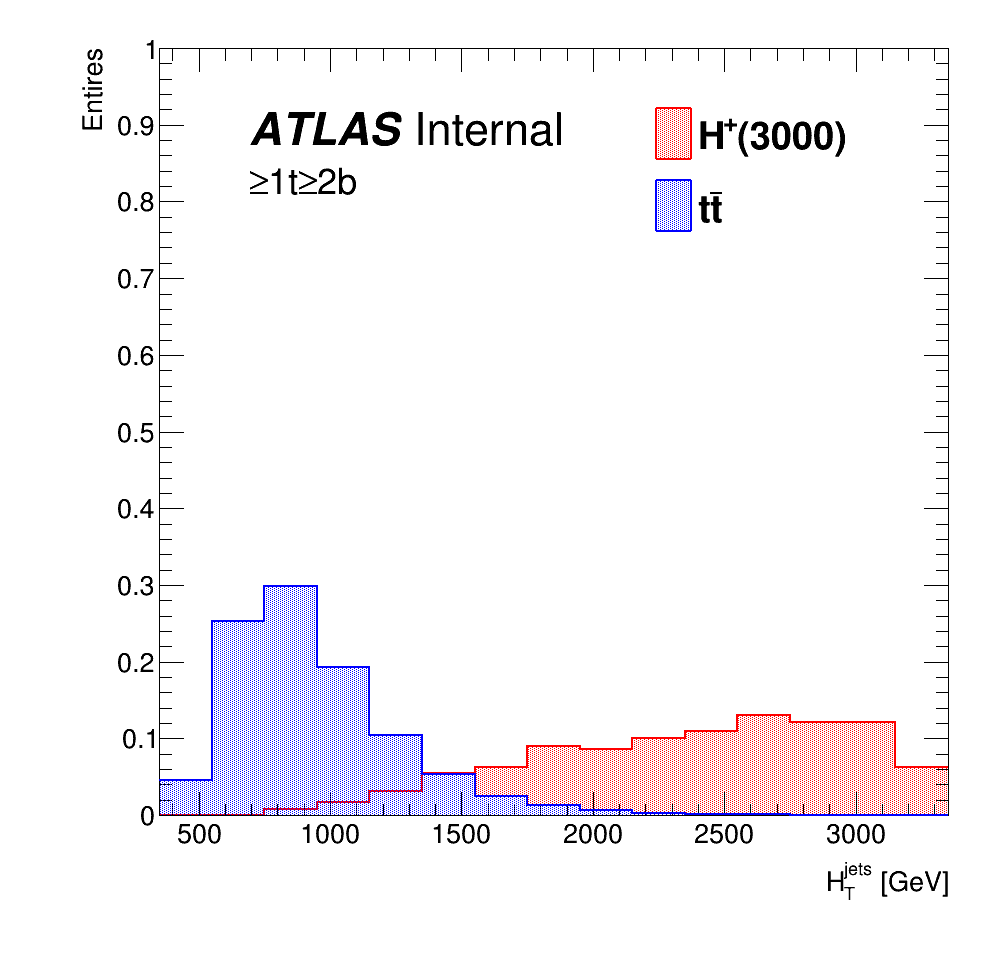
\includegraphics[width=0.25\textwidth]{images/AnalysisStrategy/SOVERB_Hp3000_Contained80_DL1r_70_HT_jets_Contained80_DL1r_70.png}
        \label{fig:SOVERB_HT_jets_Hp3000_Contained80_DL1r_70}
      }
      \subfloat[LeadingJet\_pt] {
        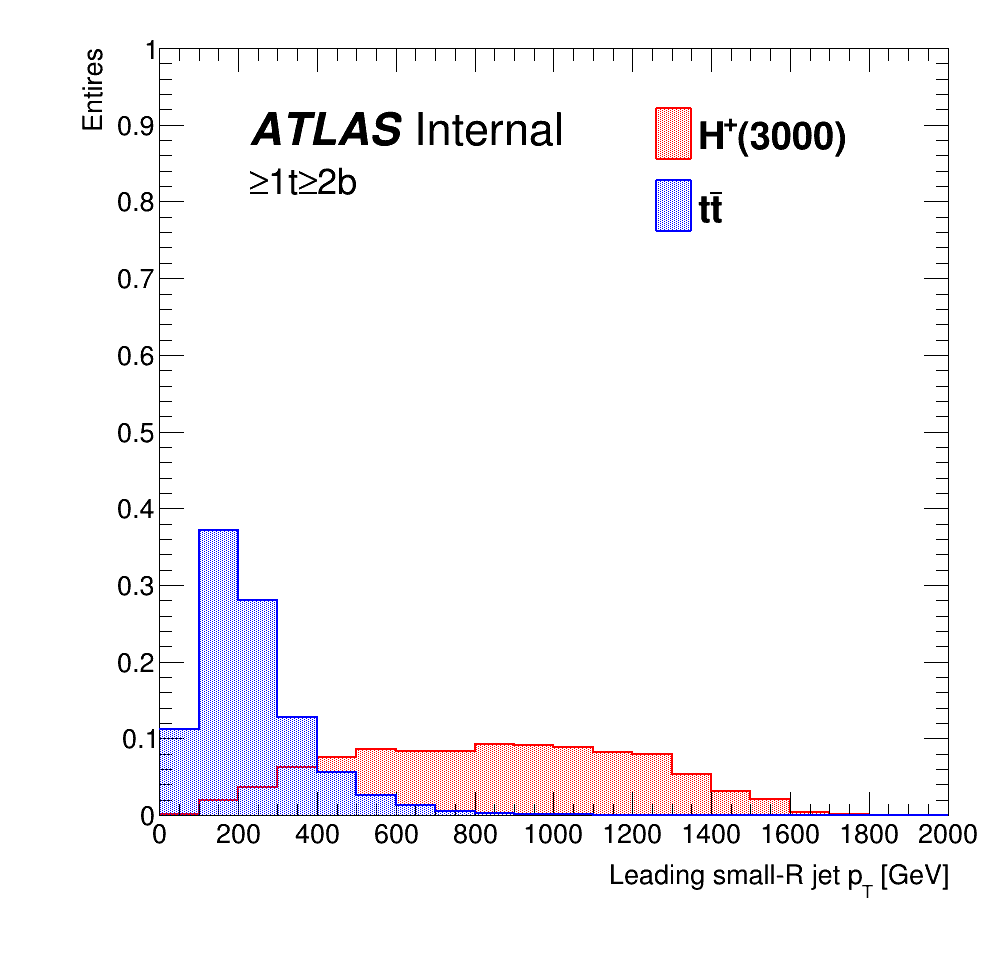
\includegraphics[width=0.25\textwidth]{images/AnalysisStrategy/SOVERB_Hp3000_Contained80_DL1r_70_leadingJet_pt_Contained80_DL1r_70.png}
        \label{fig:SOVERB_LeadingJet_pt_Hp3000_Contained80_DL1r_70}
      }
      \subfloat[Centrality\_all] {
        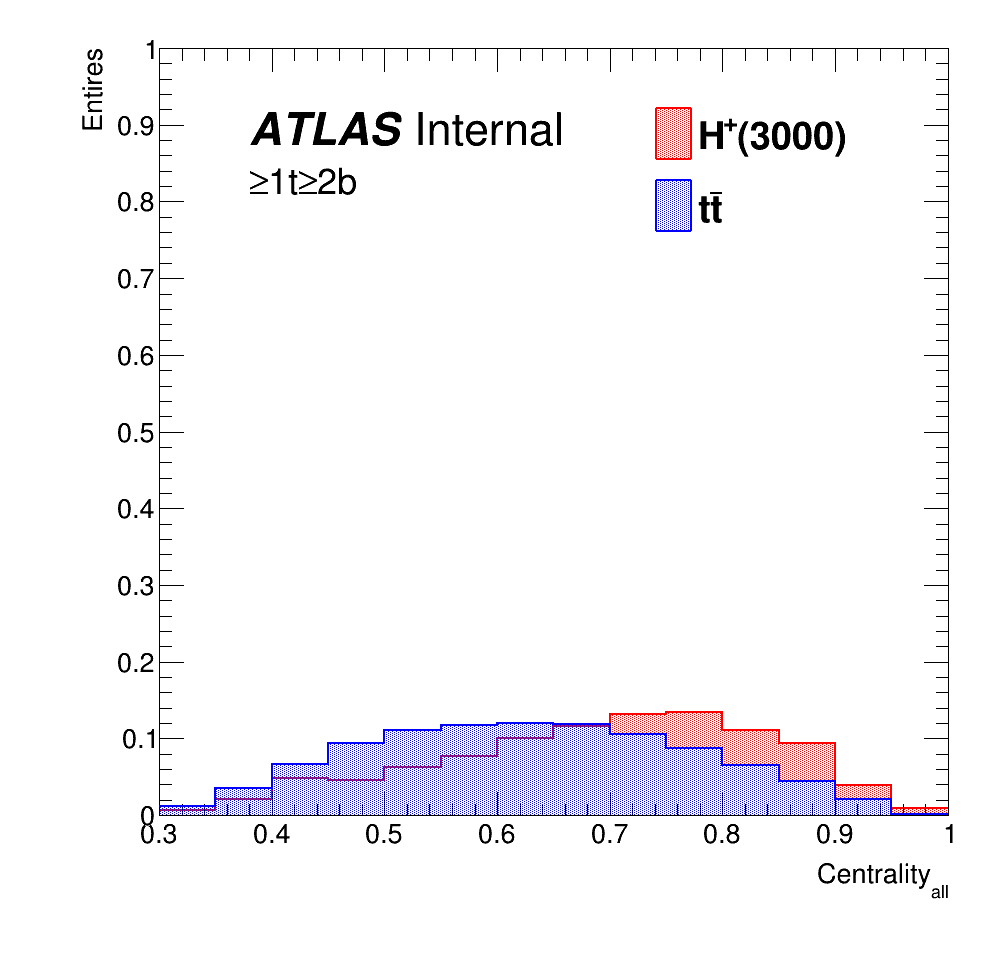
\includegraphics[width=0.25\textwidth]{images/AnalysisStrategy/SOVERB_Hp3000_Contained80_DL1r_70_Centrality_all_Contained80_DL1r_70.png}
        \label{fig:SOVERB_Centrality_all_Hp3000_Contained80_DL1r_70}
      }
      \subfloat[H1\_all] {
        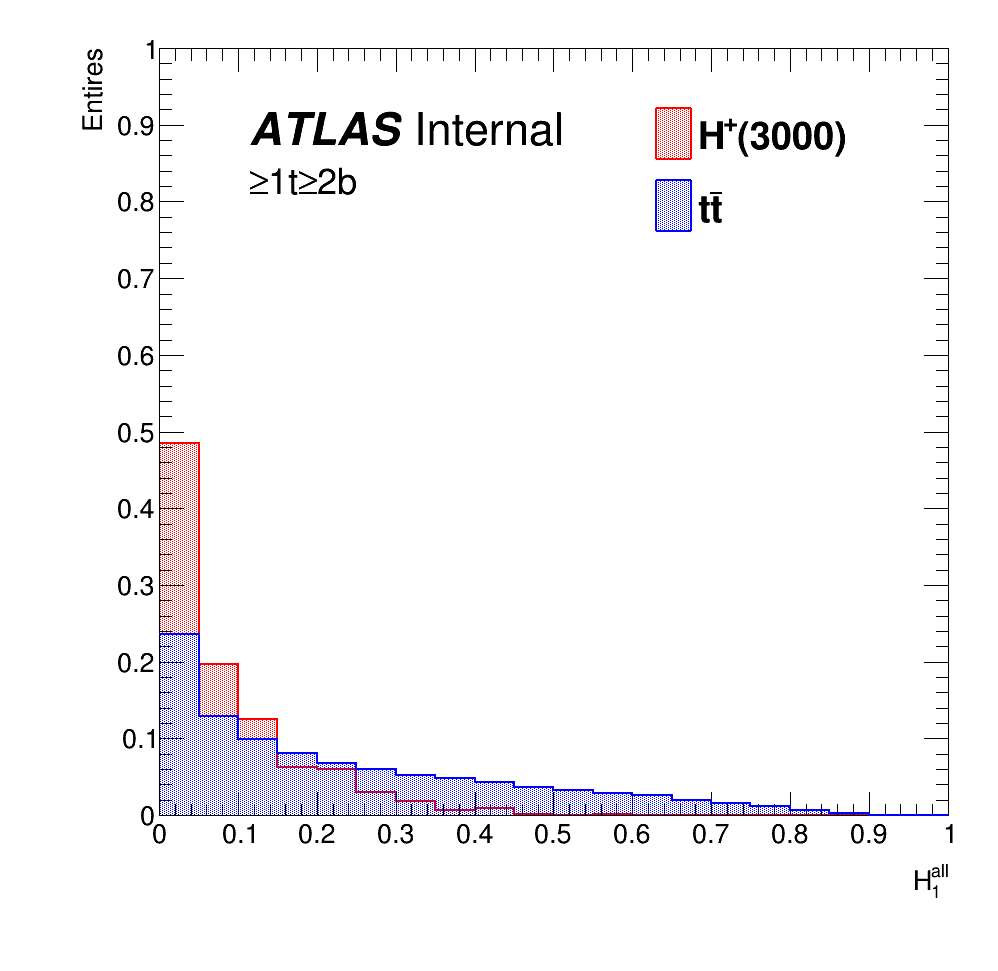
\includegraphics[width=0.25\textwidth]{images/AnalysisStrategy/SOVERB_Hp3000_Contained80_DL1r_70_H1_all_Contained80_DL1r_70.png}
        \label{fig:SOVERB_H1_all_Hp3000_Contained80_DL1r_70}
      }\\
      \subfloat[Mbb\_MaxPt] {
        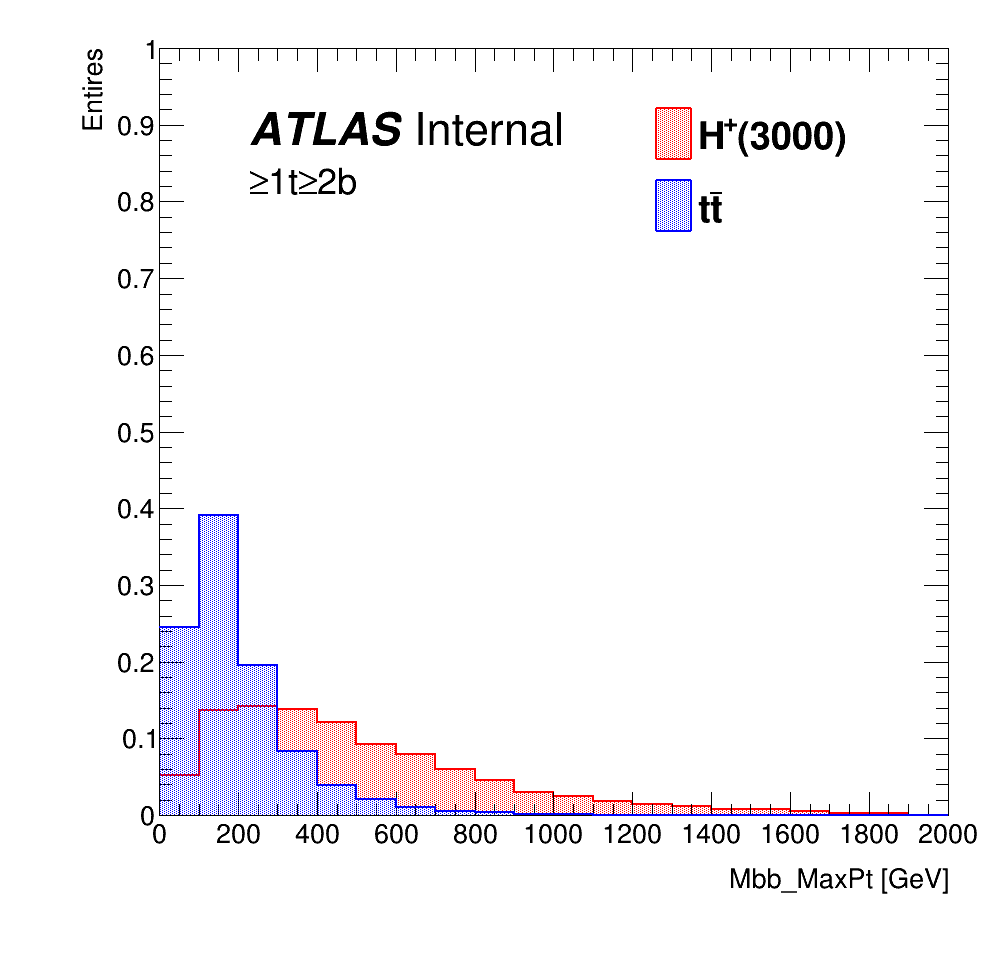
\includegraphics[width=0.25\textwidth]{images/AnalysisStrategy/SOVERB_Hp3000_Contained80_DL1r_70_Mbb_MaxPt_Contained80_DL1r_70.png}
        \label{fig:SOVERB_Mbb_MaxPt_Hp3000_Contained80_DL1r_70}
      }
      \subfloat[Mjjj\_MaxPt] {
        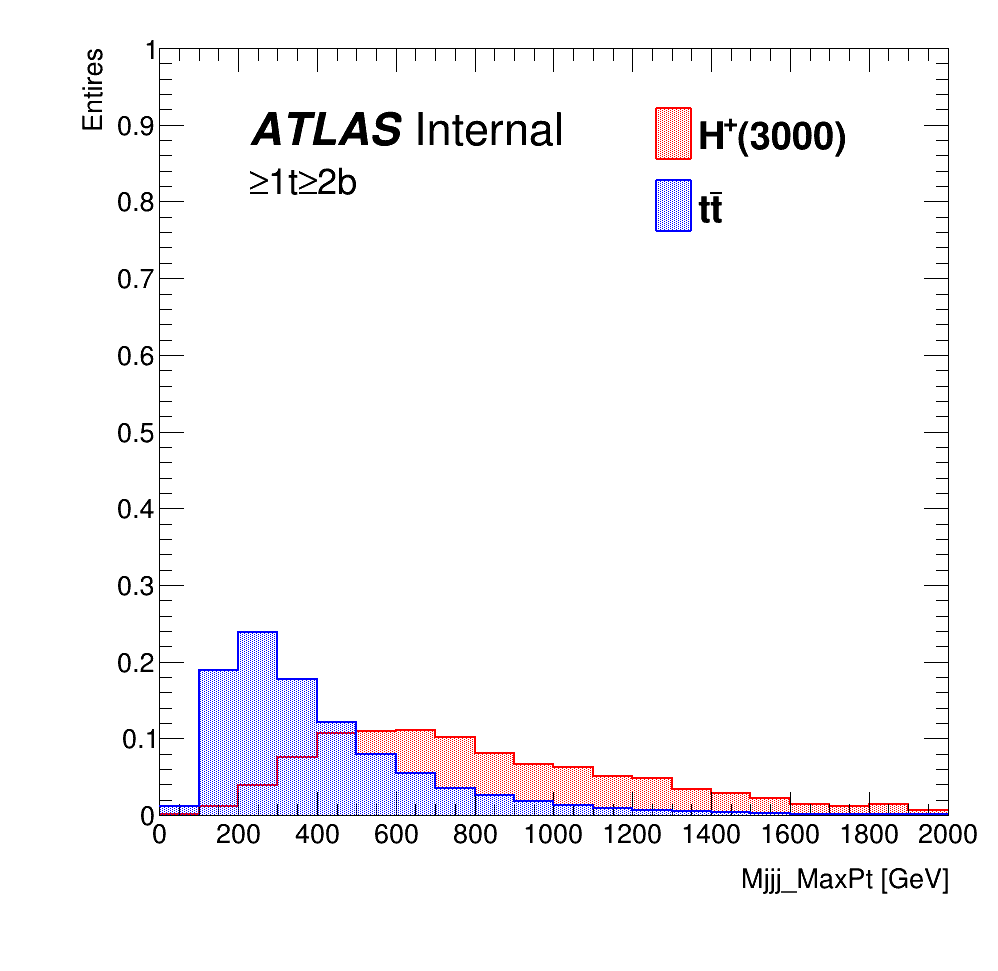
\includegraphics[width=0.25\textwidth]{images/AnalysisStrategy/SOVERB_Hp3000_Contained80_DL1r_70_Mjjj_MaxPt_Contained80_DL1r_70.png}
        \label{fig:SOVERB_Mjjj_MaxPt_Hp3000_Contained80_DL1r_70}
      }
      \subfloat[Muu\_MindR] {
        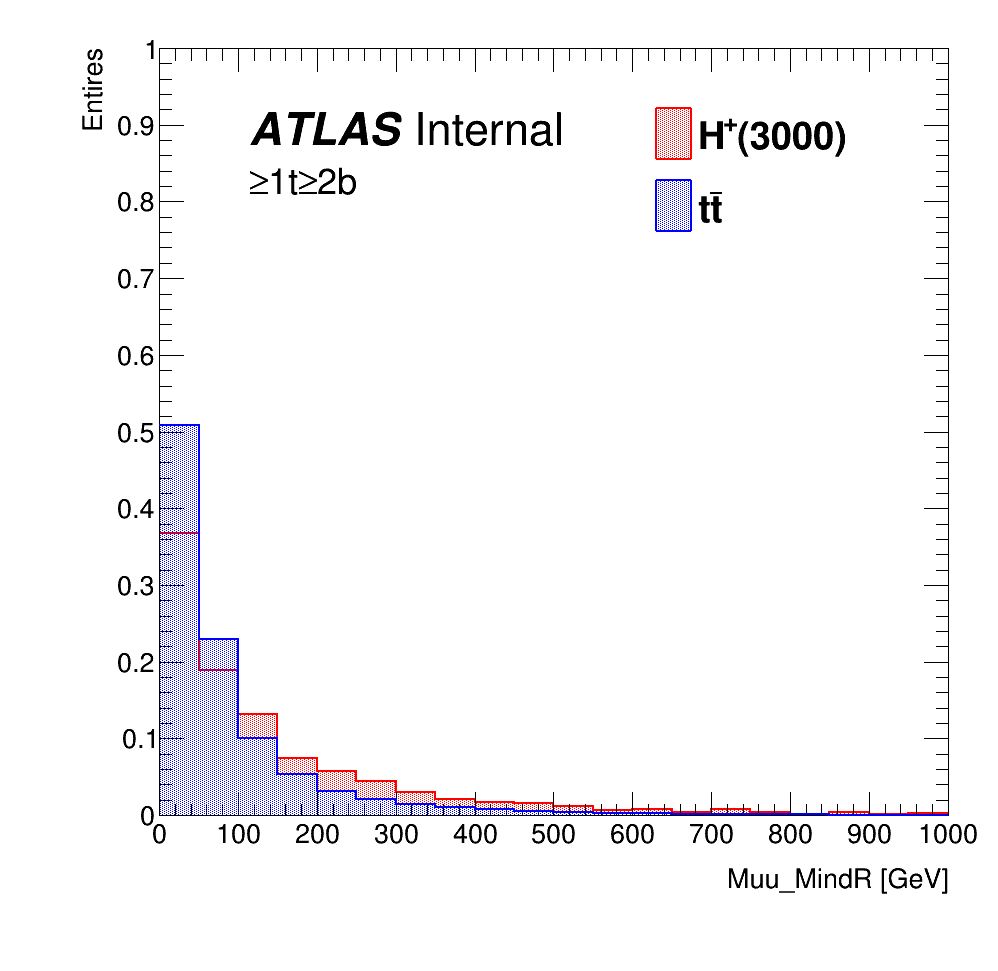
\includegraphics[width=0.25\textwidth]{images/AnalysisStrategy/SOVERB_Hp3000_Contained80_DL1r_70_Muu_MindR_Contained80_DL1r_70.png}
        \label{fig:SOVERB_Muu_MindR_Hp3000_Contained80_DL1r_70}
      }
      \subfloat[dRbb\_avg] {
        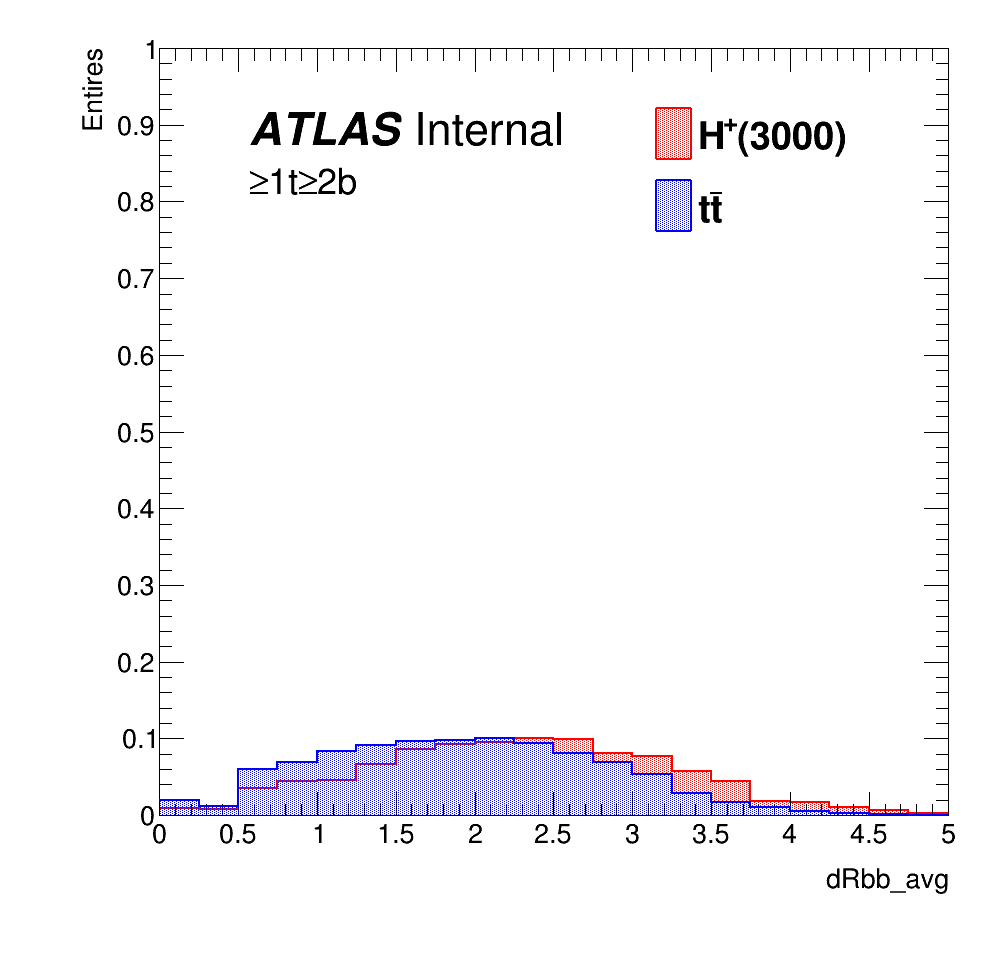
\includegraphics[width=0.25\textwidth]{images/AnalysisStrategy/SOVERB_Hp3000_Contained80_DL1r_70_dRbb_avg_Contained80_DL1r_70.png}
        \label{fig:SOVERB_dRbb_avg_Hp3000_Contained80_DL1r_70}
      }\\
      \subfloat[dRlepbb\_MindR] {
        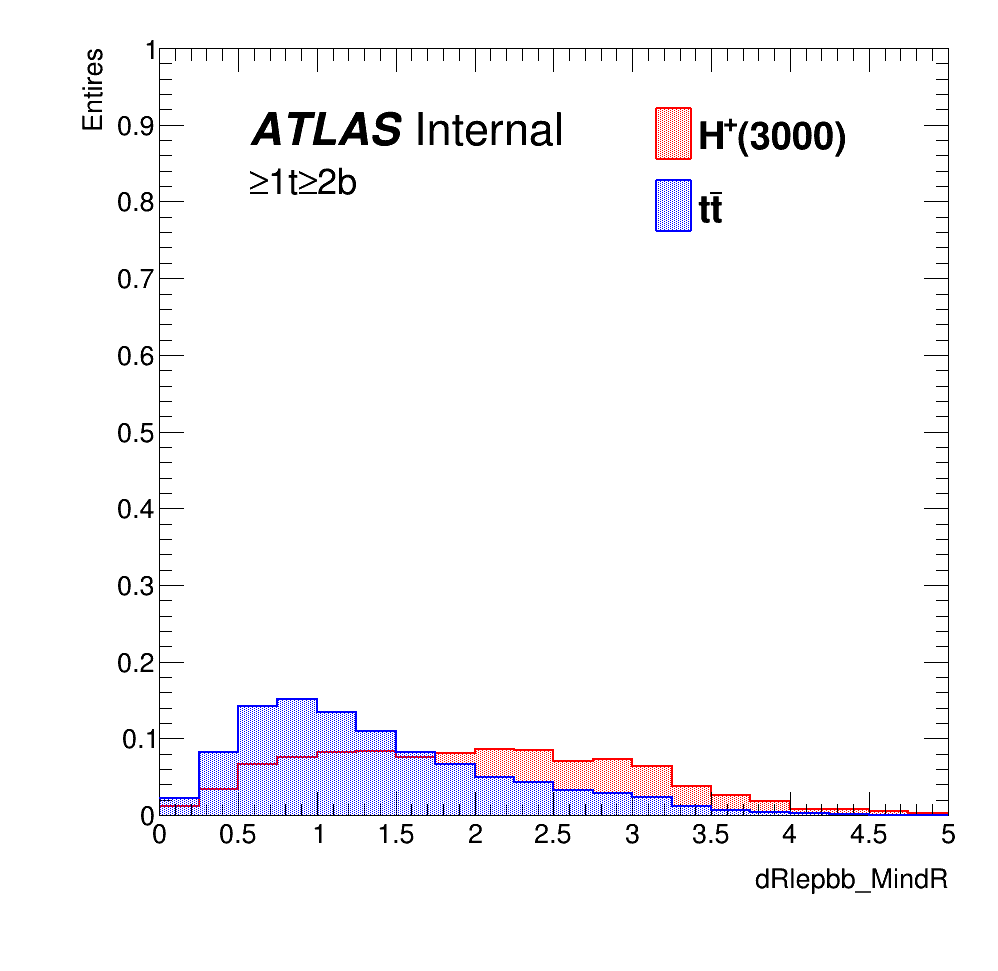
\includegraphics[width=0.25\textwidth]{images/AnalysisStrategy/SOVERB_Hp3000_Contained80_DL1r_70_dRlepbb_MindR_Contained80_DL1r_70.png}
        \label{fig:SOVERB_dRlepbb_MindR_Hp3000_Contained80_DL1r_70}
      }
      \subfloat[LeadingTop\_m] {
        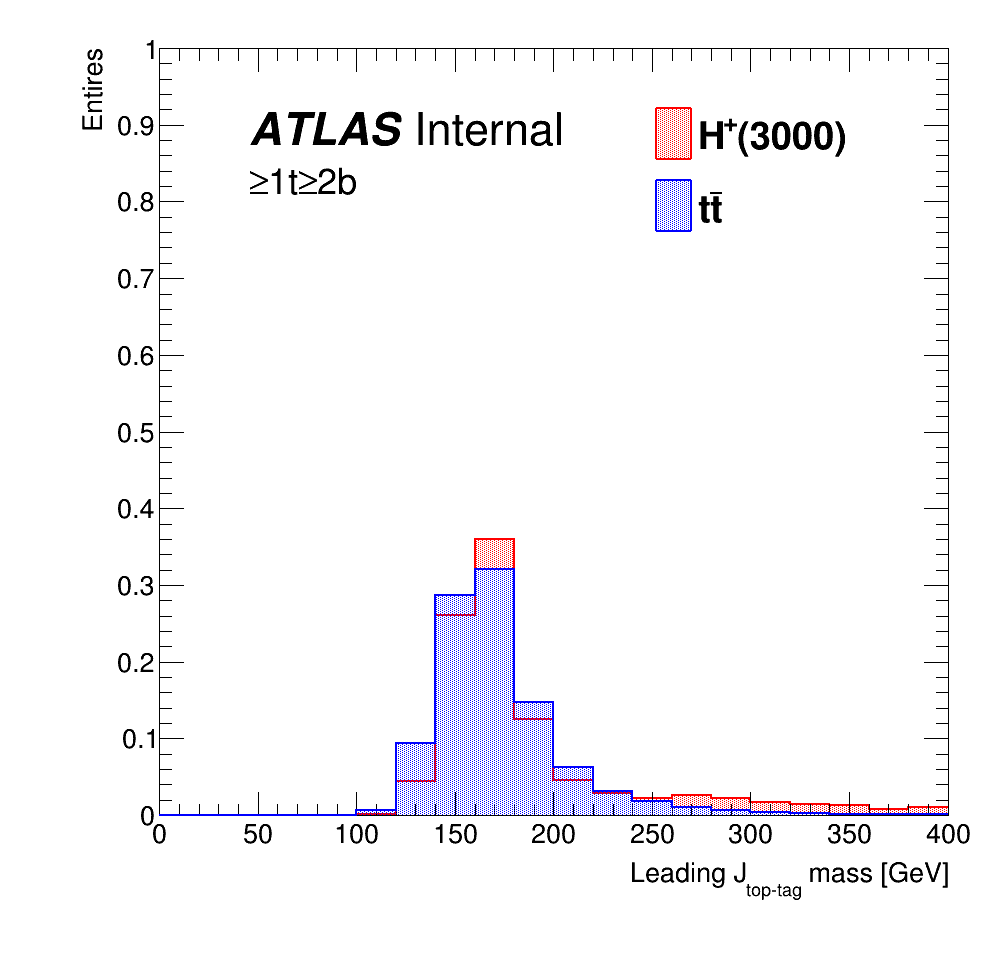
\includegraphics[width=0.25\textwidth]{images/AnalysisStrategy/SOVERB_Hp3000_Contained80_DL1r_70_leadingTop_m_Contained80_DL1r_70.png}
        \label{fig:SOVERB_leadingTop_mass_Hp3000_Contained80_DL1r_70}
      }
      \subfloat[LeadingTop\_pt] {
        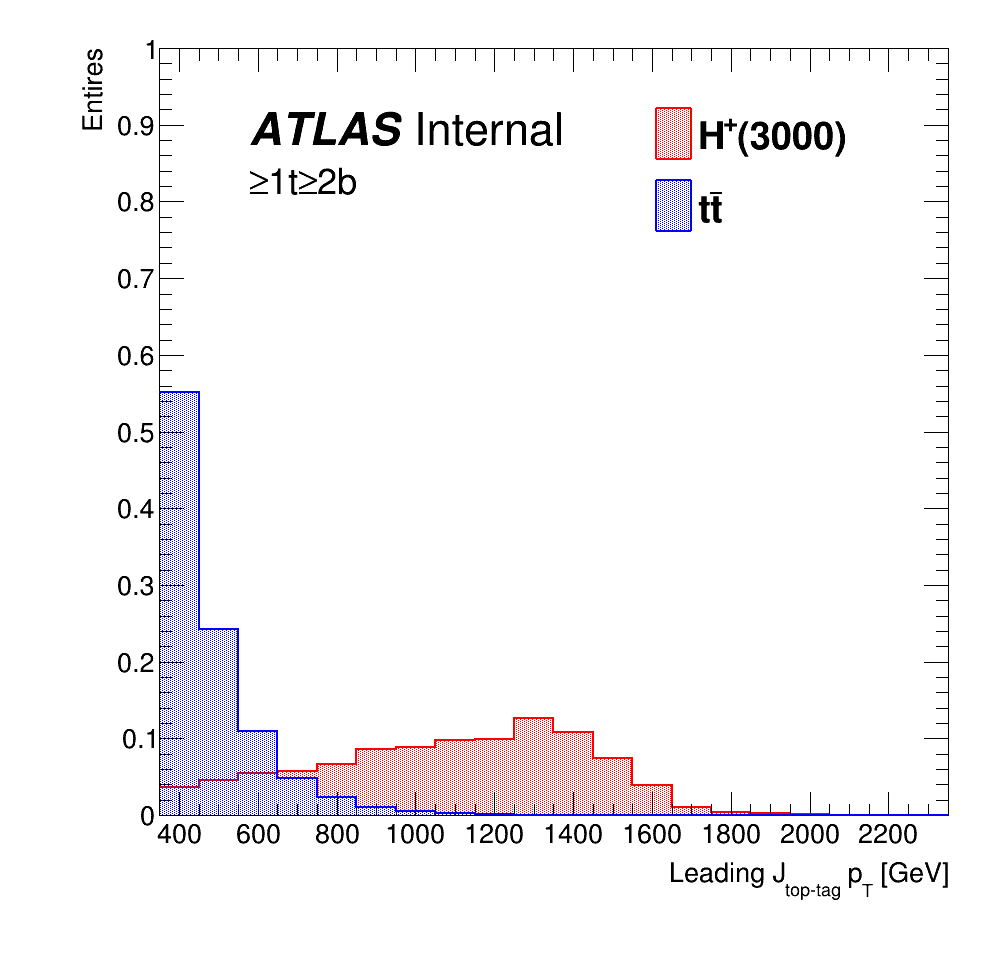
\includegraphics[width=0.25\textwidth]{images/AnalysisStrategy/SOVERB_Hp3000_Contained80_DL1r_70_leadingTop_pt_Contained80_DL1r_70.png}
        \label{fig:SOVERB_leadingTop_pt_Hp3000_Contained80_DL1r_70}
      }
      \subfloat[M\_tb] {
        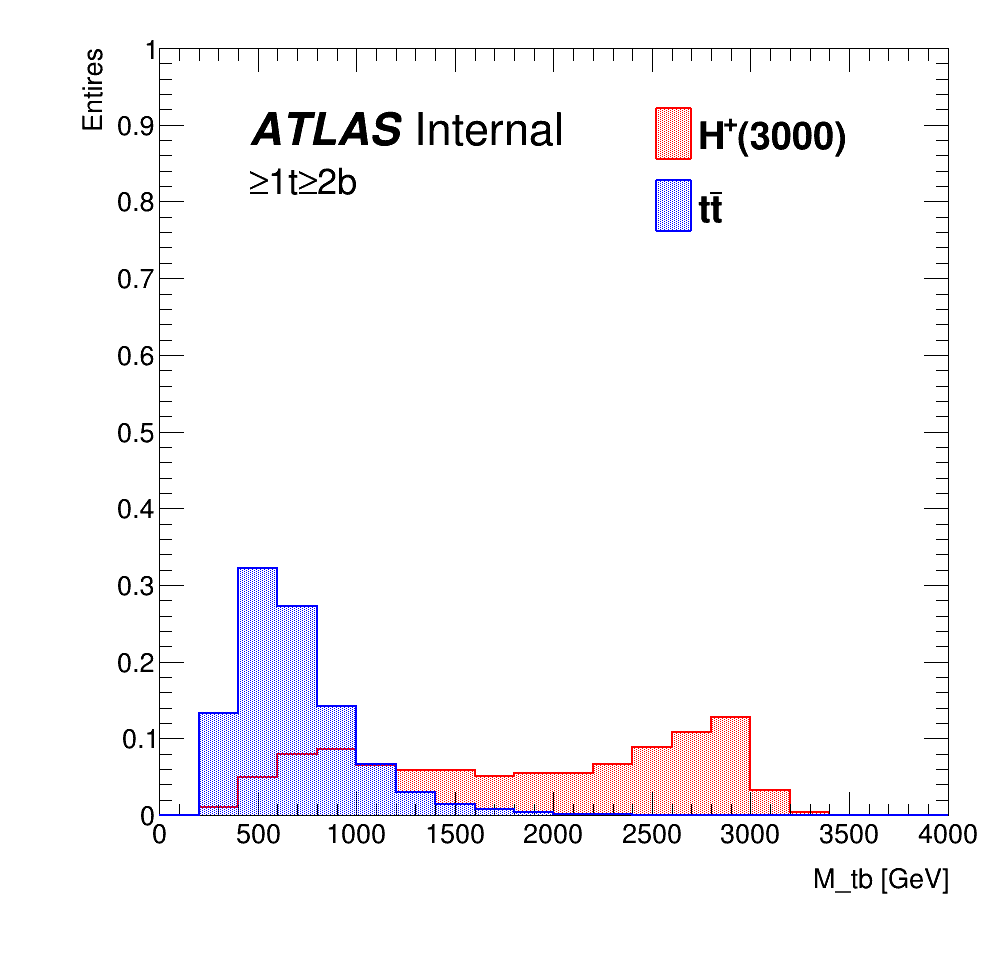
\includegraphics[width=0.25\textwidth]{images/AnalysisStrategy/SOVERB_Hp3000_Contained80_DL1r_70_tb_m_Contained80_DL1r_70.png}
        \label{fig:SOVERB_M_tb_Hp3000_Contained80_DL1r_70}
      }\\
      \subfloat[Pt\_tb] {
        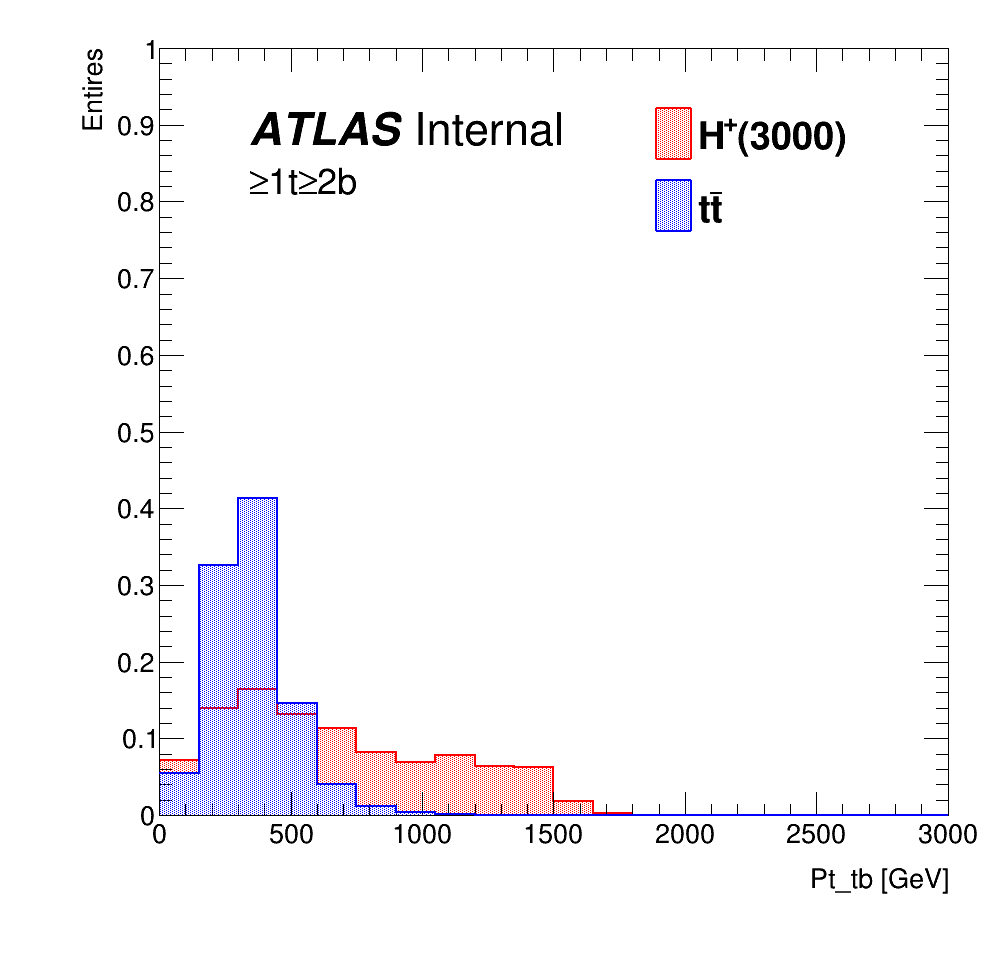
\includegraphics[width=0.25\textwidth]{images/AnalysisStrategy/SOVERB_Hp3000_Contained80_DL1r_70_tb_pt_Contained80_DL1r_70.png}
        \label{fig:SOVERB_Pt_tb_Hp3000_Contained80_DL1r_70}
      }
      \caption{Comparison of input variables for BDT training between $H^{+}$ and $t\bar{t}+\text{jets}$ events under 3000 GeV $H^{+}$ mass hypothesis in the inclusive SR (i.e, SR1 + SR2).}
      \label{fig:SOVERB_Hp3000_Contained80_DL1r_70}
    \end{figure}

    \item{\textbf{Results of BDT training}}\mbox{}\\
    The BDT output distributions for $H^{+}$ signal and background events in the inclusive SR region (i.e., SR1+SR2) for different values of the $H^+$ mass are shown in Figure \ref{fig:BDTTrainingResults_Hp1000} to \ref{fig:BDTTrainingResults_Hp3000}, together with receiver operating characteristic (ROC) curves.

    %--- BDT template H+(1000)
    \begin{figure}[H]
      \centering
      \subfloat[BDT output]{
        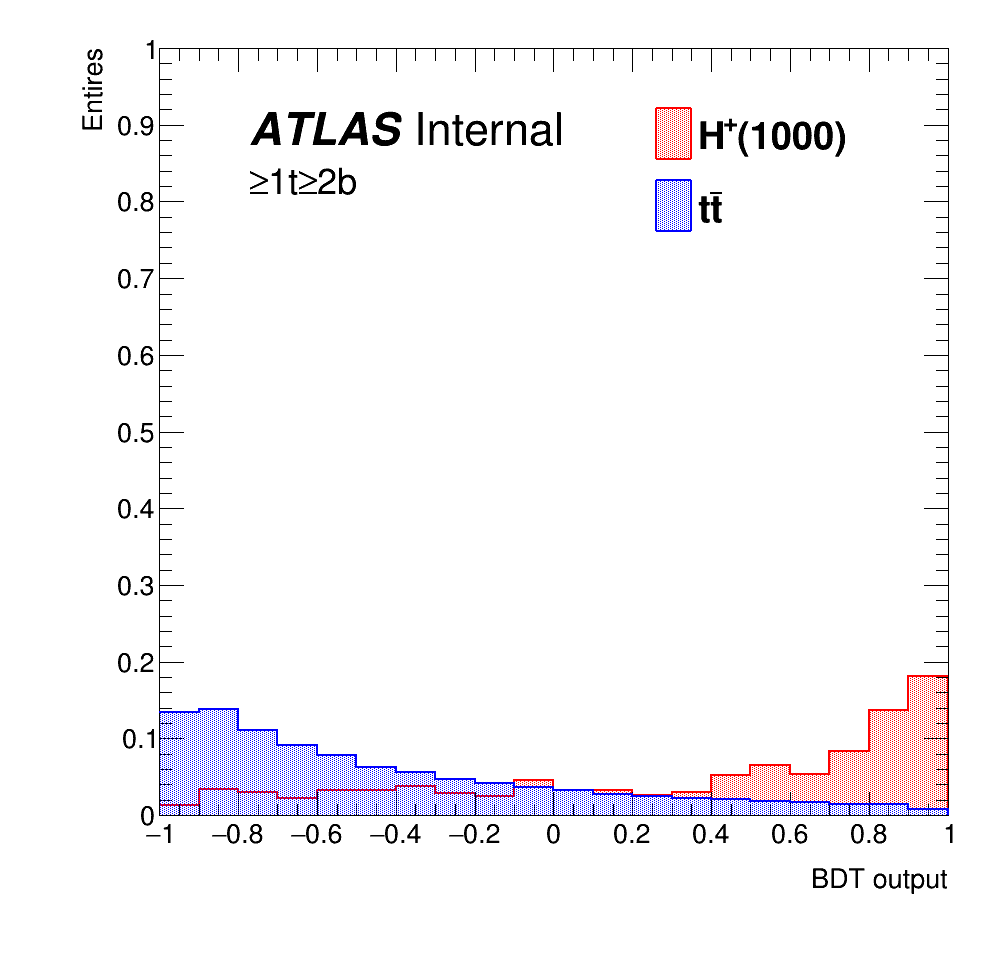
\includegraphics[width=0.45\textwidth]{images/AnalysisStrategy/BDTOutput_Hp1000_Contained80_DL1r_70.png}
        \label{fig:BDTOutput_Hp1000}
      }
      \subfloat[ROC curve]{
        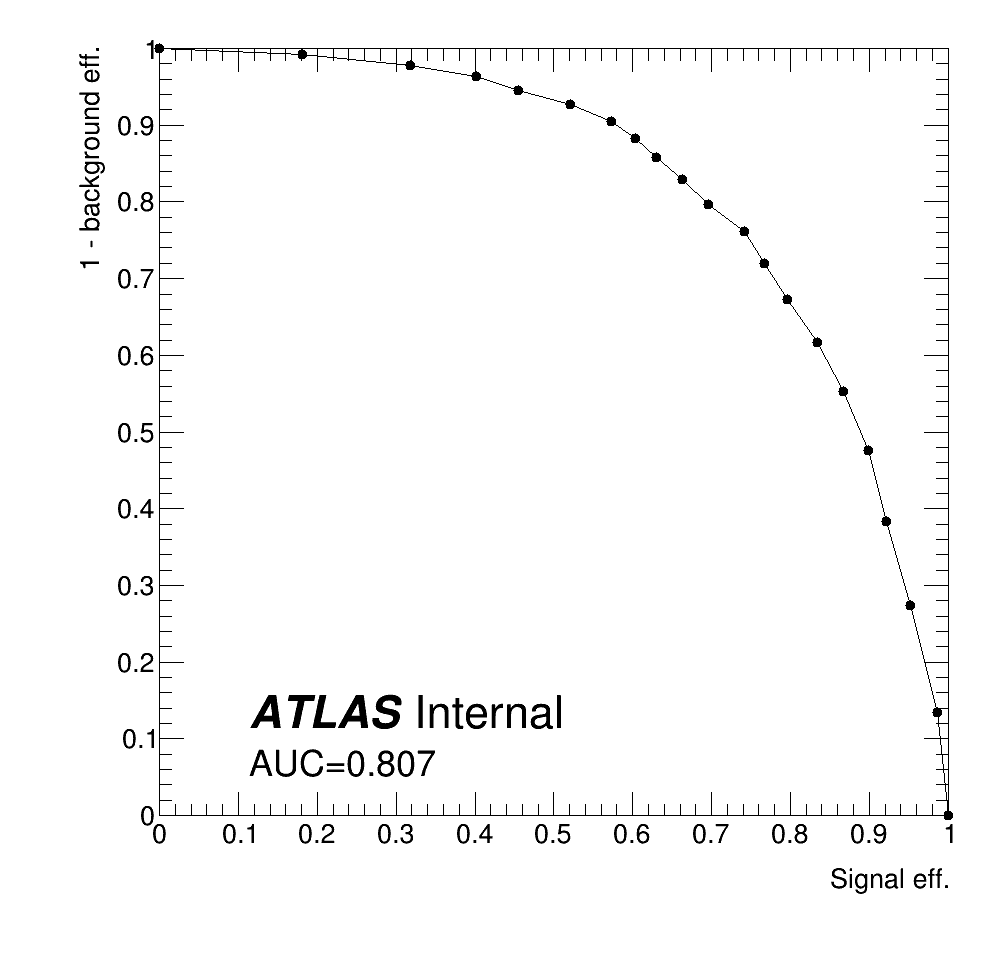
\includegraphics[width=0.45\textwidth]{images/AnalysisStrategy/ROCCurve_Hp1000_Contained80_DL1r_70.png}
        \label{fig:ROCCurve_Hp1000}
      }
      \caption{BDT distribution and ROC curve for the 1000 GeV $H^{+}$ mass hypothesis.}
      \label{fig:BDTTrainingResults_Hp1000}
    \end{figure}
    
    %--- BDT template H+(1200)
    \begin{figure}[H]
      \centering
      \subfloat[BDT output]{
        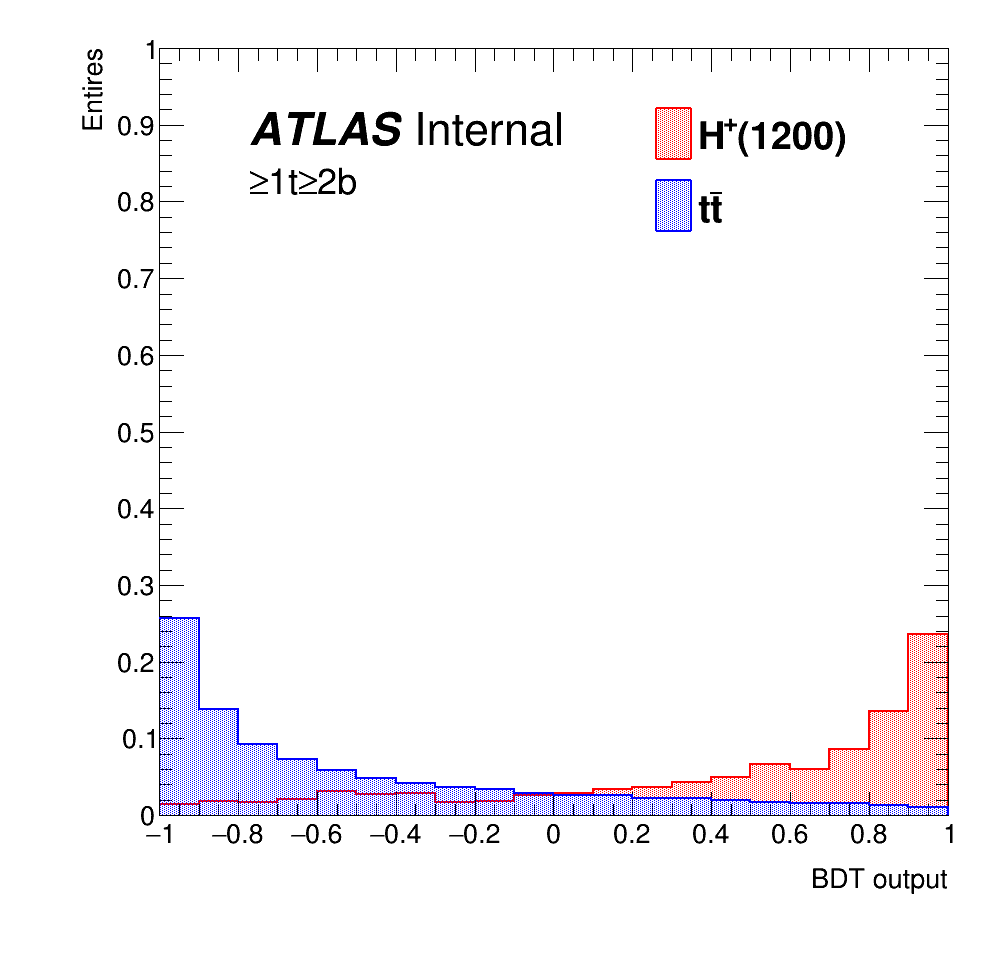
\includegraphics[width=0.45\textwidth]{images/AnalysisStrategy/BDTOutput_Hp1200_Contained80_DL1r_70.png}
        \label{fig:BDTOutput_Hp1200}
      }
      \subfloat[ROC curve]{
        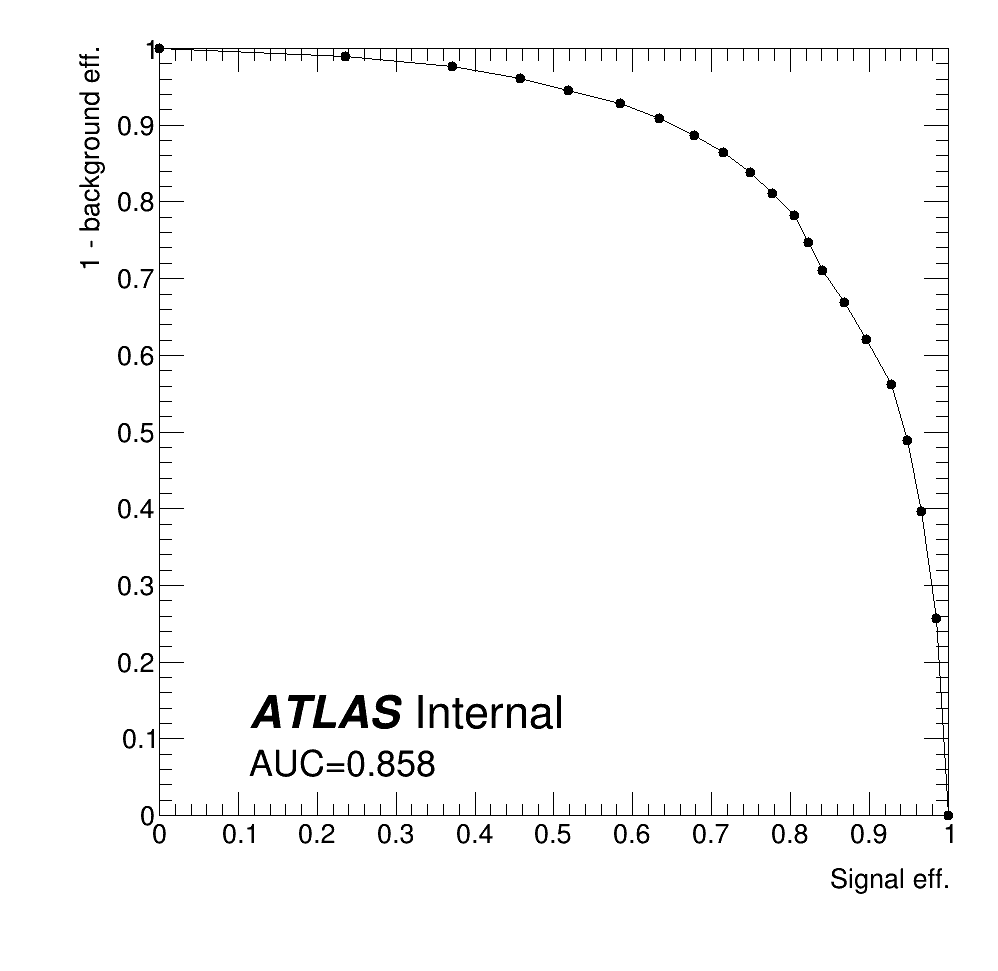
\includegraphics[width=0.45\textwidth]{images/AnalysisStrategy/ROCCurve_Hp1200_Contained80_DL1r_70.png}
        \label{fig:ROCCurve_Hp1200}
      }
      \caption{BDT distribution and ROC curve for the 1200 GeV $H^{+}$ mass hypothesis.}
      \label{fig:BDTTrainingResults_Hp1200}
    \end{figure}
    
    %--- BDT template H+(1400)
    \begin{figure}[H]
      \centering
      \subfloat[BDT output]{
        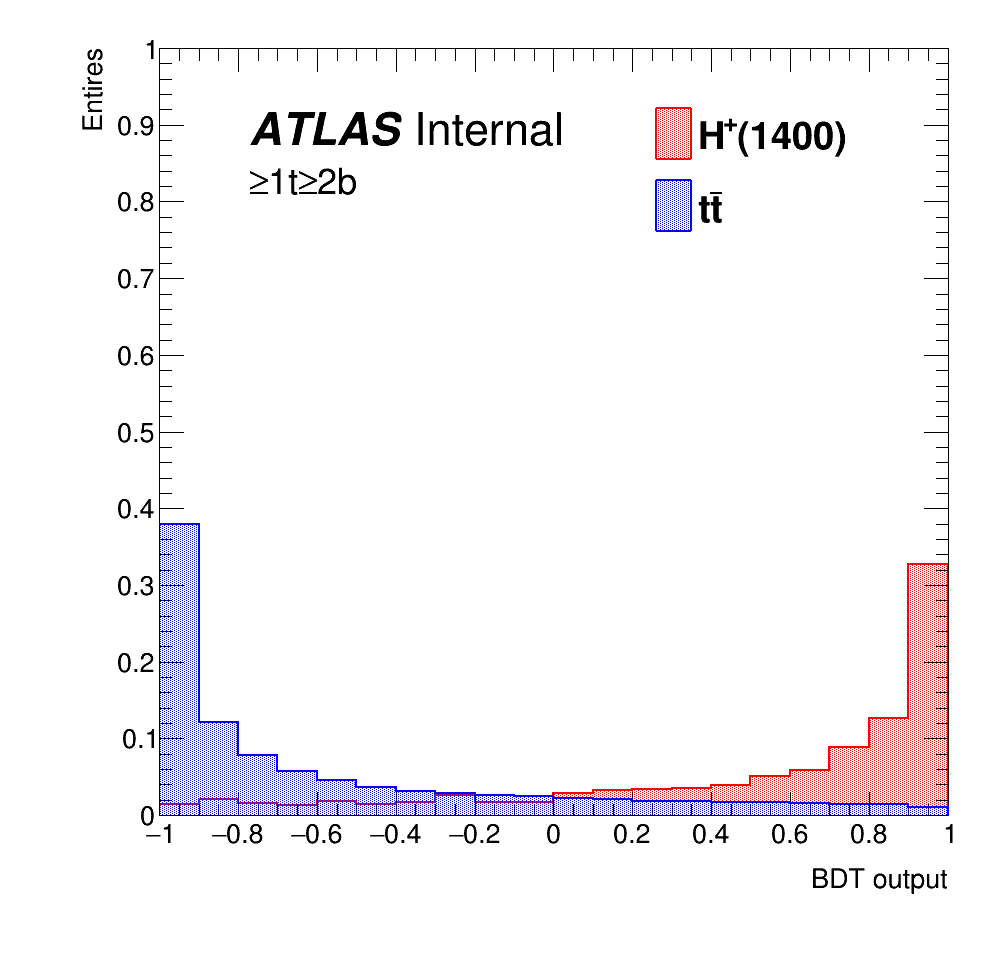
\includegraphics[width=0.45\textwidth]{images/AnalysisStrategy/BDTOutput_Hp1400_Contained80_DL1r_70.png}
        \label{fig:BDTOutput_Hp1400}
      }
      \subfloat[ROC curve]{
        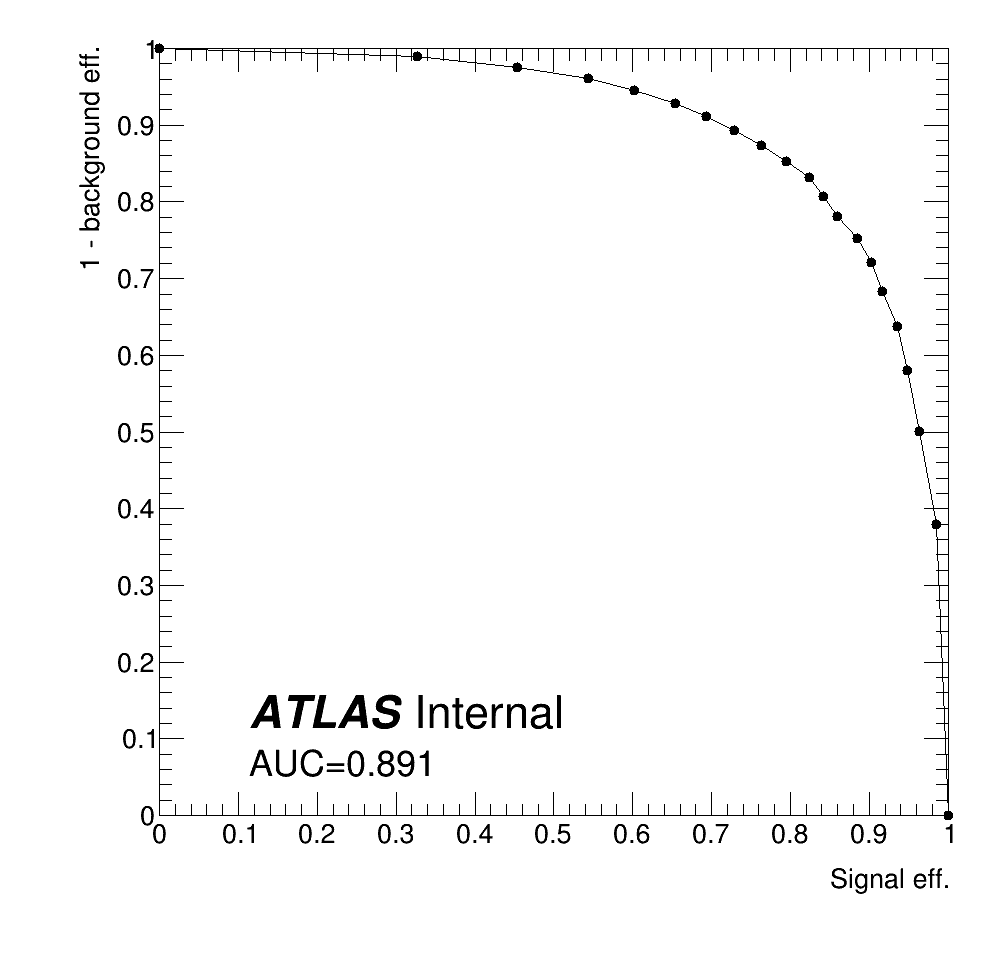
\includegraphics[width=0.45\textwidth]{images/AnalysisStrategy/ROCCurve_Hp1400_Contained80_DL1r_70.png}
        \label{fig:ROCCurve_Hp1400}
      }
      \caption{BDT distribution and ROC curve for the 1400 GeV $H^{+}$ mass hypothesis.}
      \label{fig:BDTTrainingResults_Hp1400}
    \end{figure}
    
    %--- BDT template H+(1600)
    \begin{figure}[H]
      \centering
      \subfloat[BDT output]{
        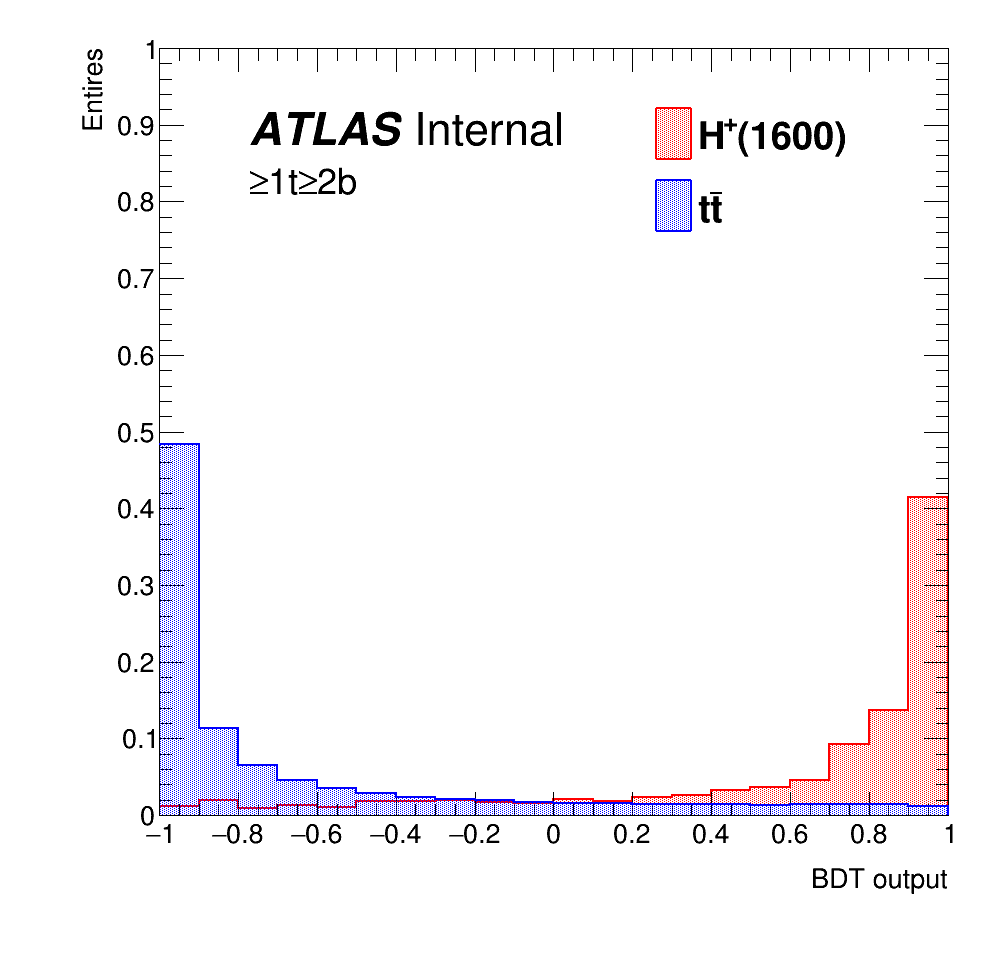
\includegraphics[width=0.45\textwidth]{images/AnalysisStrategy/BDTOutput_Hp1600_Contained80_DL1r_70.png}
        \label{fig:BDTOutput_Hp1600}
      }
      \subfloat[ROC curve]{
        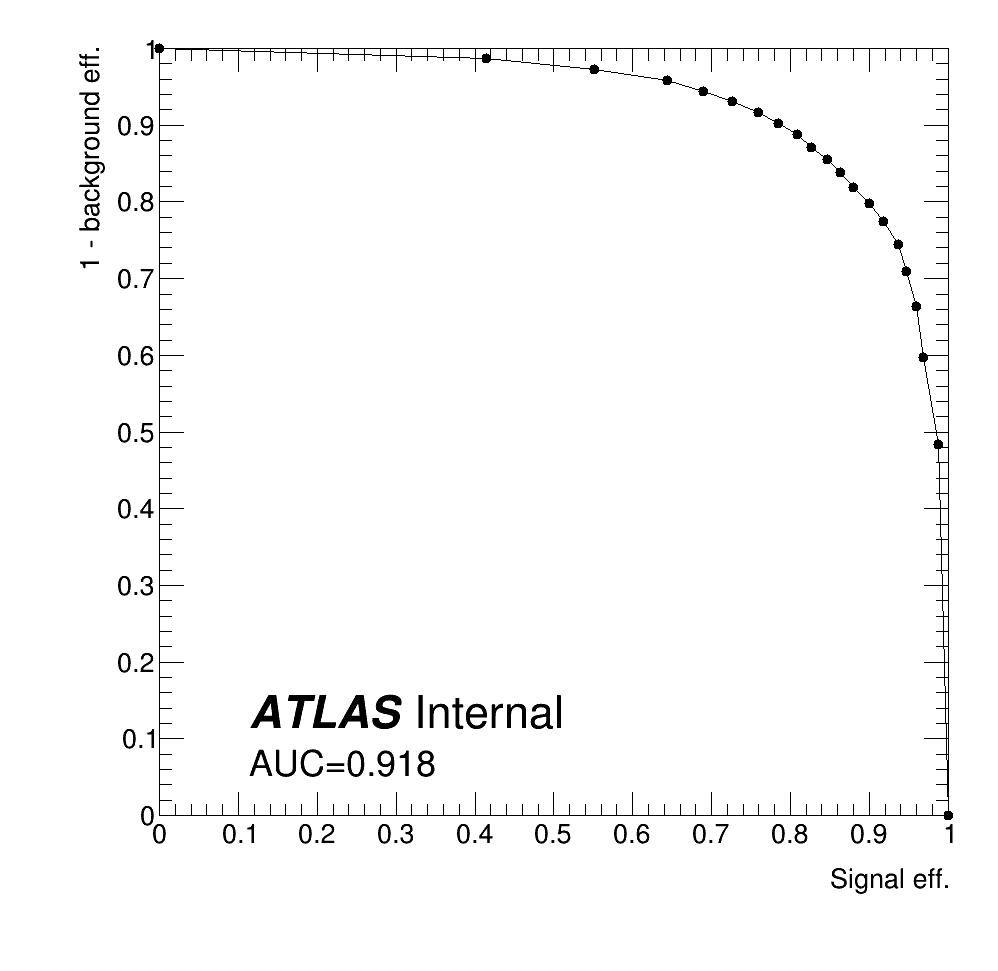
\includegraphics[width=0.45\textwidth]{images/AnalysisStrategy/ROCCurve_Hp1600_Contained80_DL1r_70.png}
        \label{fig:ROCCurve_Hp1600}
      }
      \caption{BDT distribution and ROC curve for the 1600 GeV $H^{+}$ mass hypothesis.}
      \label{fig:BDTTrainingResults_Hp1600}
    \end{figure}
    
    %--- BDT template H+(1800)
    \begin{figure}[H]
      \centering
      \subfloat[BDT output]{
        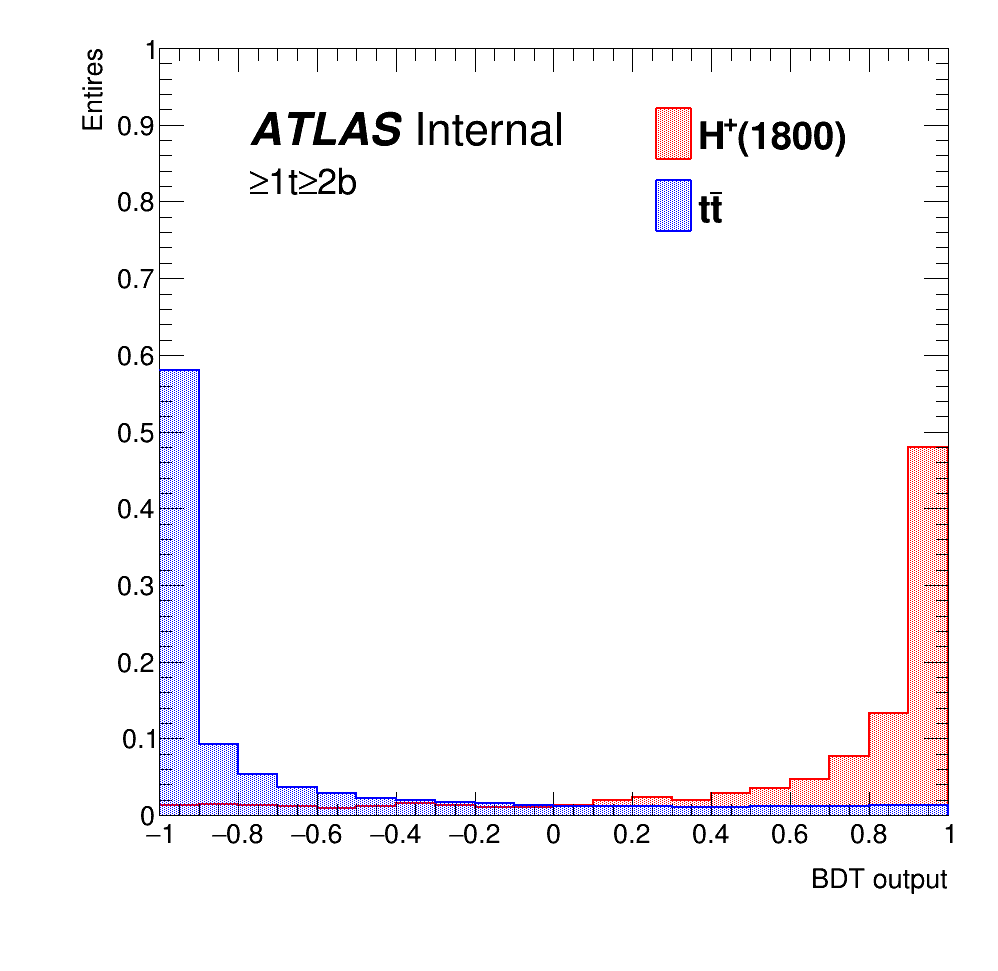
\includegraphics[width=0.45\textwidth]{images/AnalysisStrategy/BDTOutput_Hp1800_Contained80_DL1r_70.png}
        \label{fig:BDTOutput_Hp1800}
      }
      \subfloat[ROC curve]{
        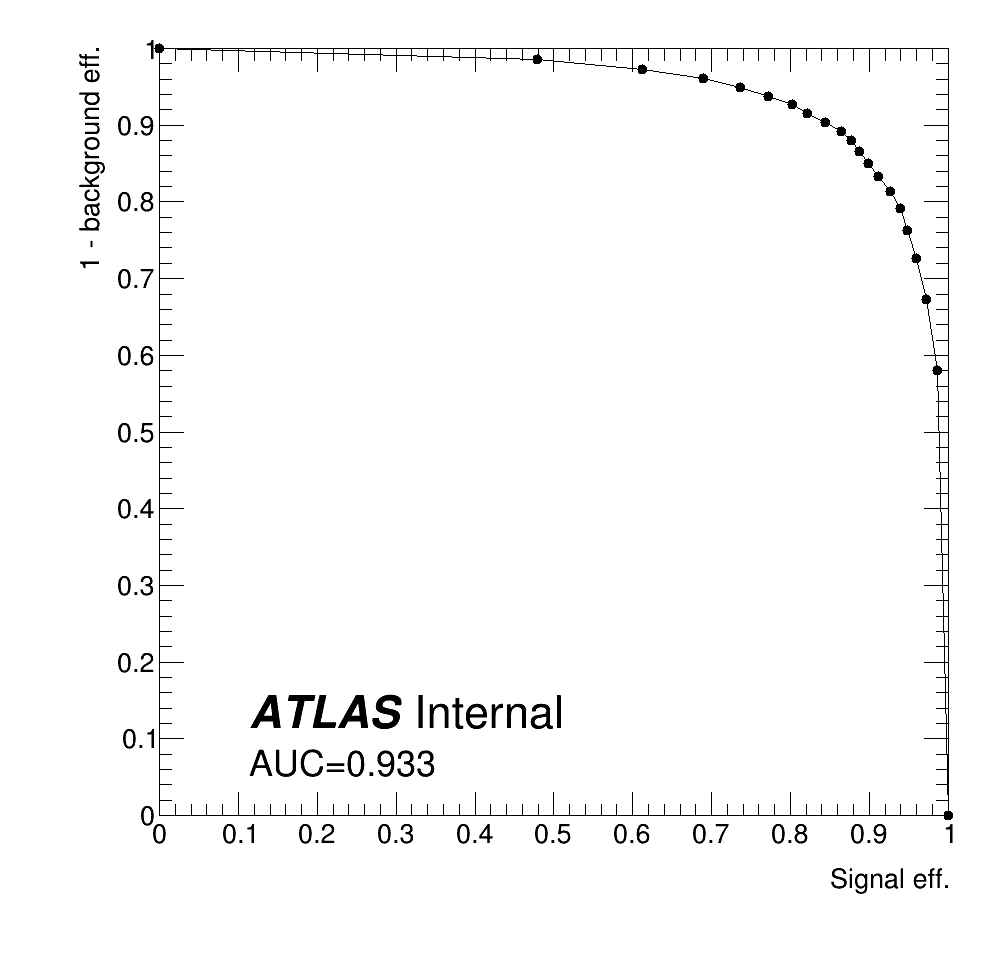
\includegraphics[width=0.45\textwidth]{images/AnalysisStrategy/ROCCurve_Hp1800_Contained80_DL1r_70.png}
        \label{fig:ROCCurve_Hp1800}
      }
      \caption{BDT distribution and ROC curve for the 1800 GeV $H^{+}$ mass hypothesis.}
      \label{fig:BDTTrainingResults_Hp1800}
    \end{figure}
    
    %--- BDT template H+(2000)
    \begin{figure}[H]
      \centering
      \subfloat[BDT output]{
        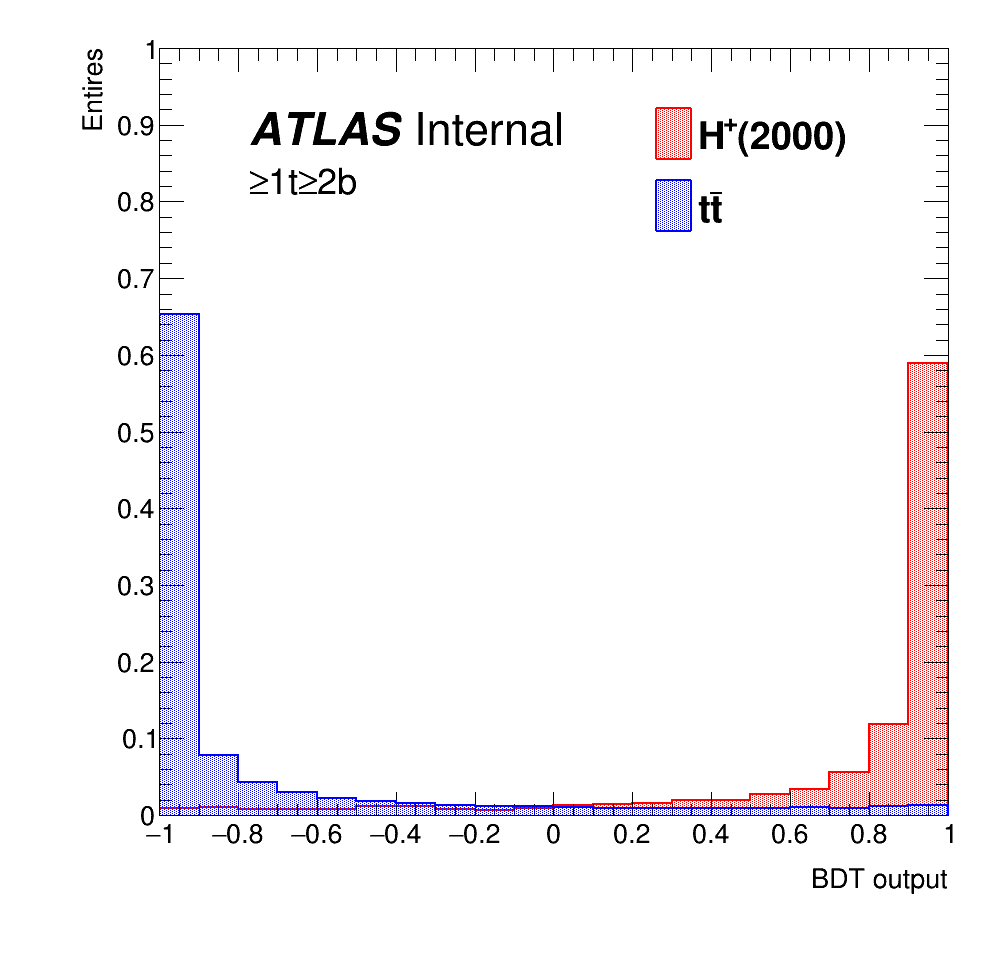
\includegraphics[width=0.45\textwidth]{images/AnalysisStrategy/BDTOutput_Hp2000_Contained80_DL1r_70.png}
        \label{fig:BDTOutput_Hp2000}
      }
      \subfloat[ROC curve]{
        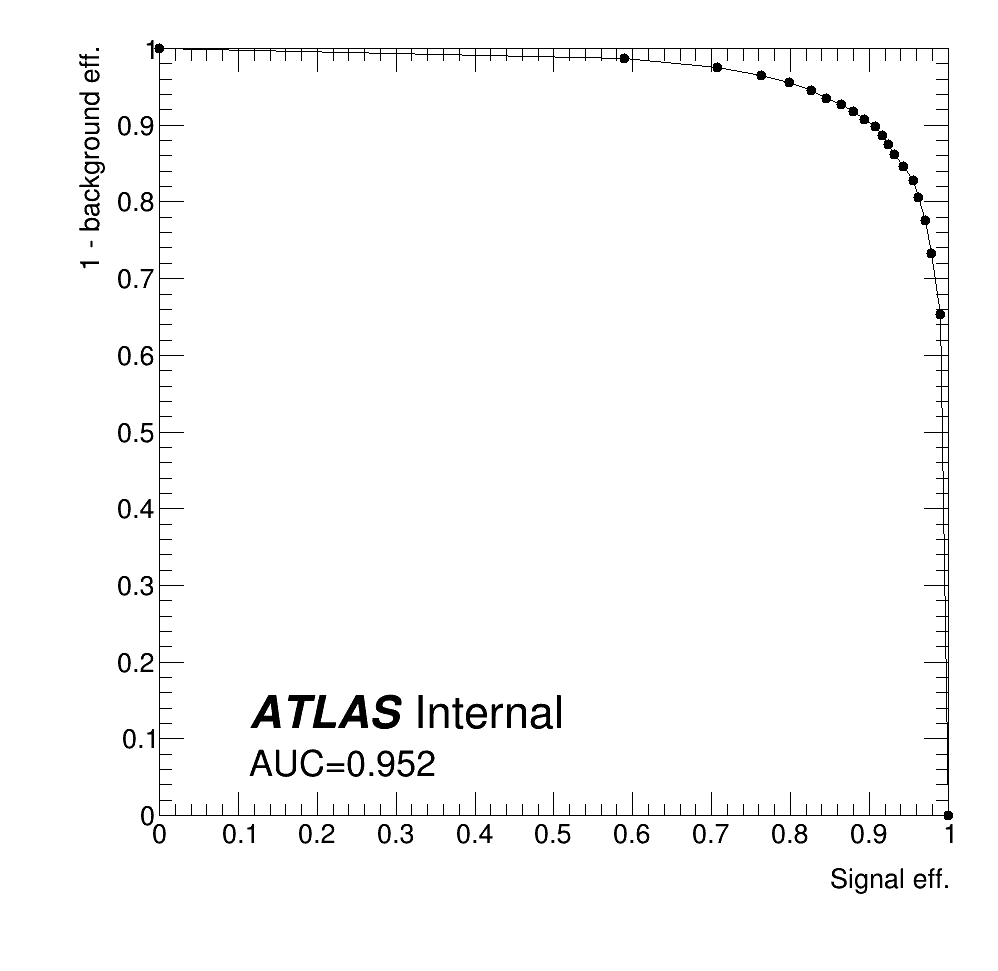
\includegraphics[width=0.45\textwidth]{images/AnalysisStrategy/ROCCurve_Hp2000_Contained80_DL1r_70.png}
        \label{fig:ROCCurve_Hp2000}
      }
      \caption{BDT distribution and ROC curve for the 2000 GeV $H^{+}$ mass hypothesis.}
      \label{fig:BDTTrainingResults_Hp2000}
    \end{figure}
    
    %--- BDT template H+(2500)
    \begin{figure}[H]
      \centering
      \subfloat[BDT output]{
        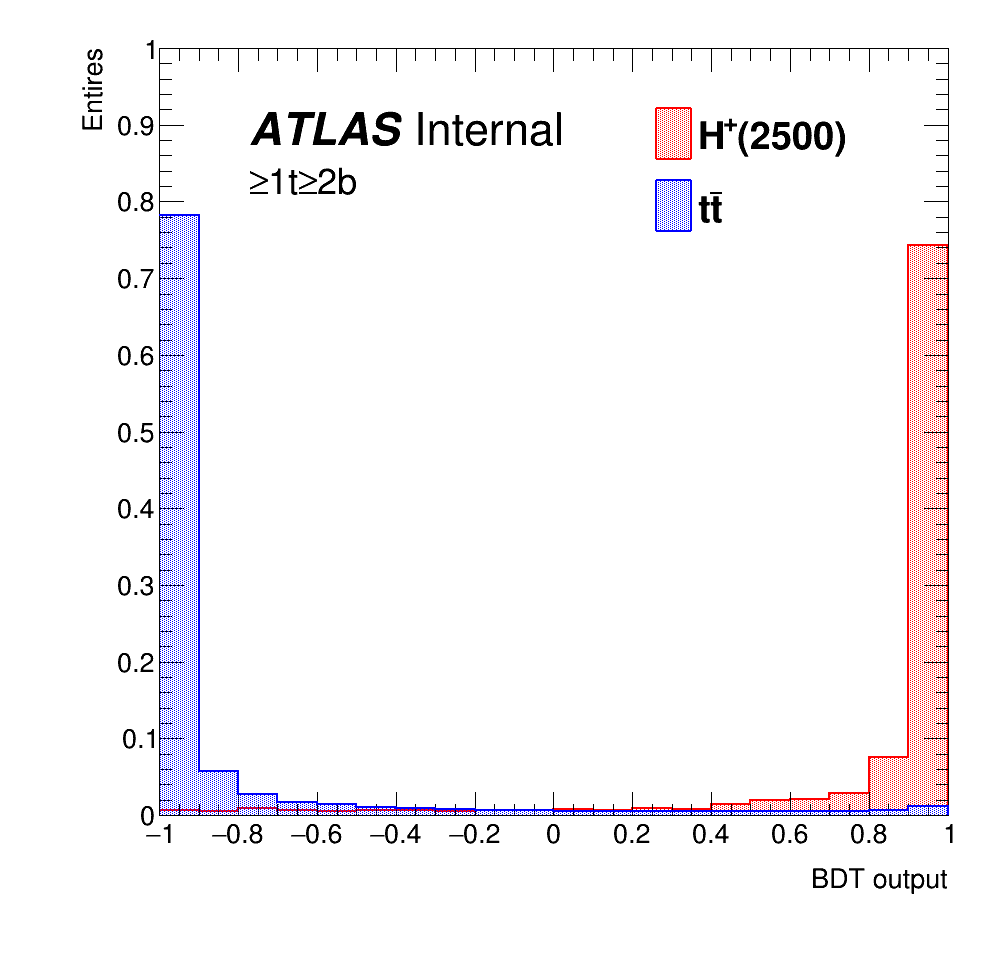
\includegraphics[width=0.45\textwidth]{images/AnalysisStrategy/BDTOutput_Hp2500_Contained80_DL1r_70.png}
        \label{fig:BDTOutput_Hp2500}
      }
      \subfloat[ROC curve]{
        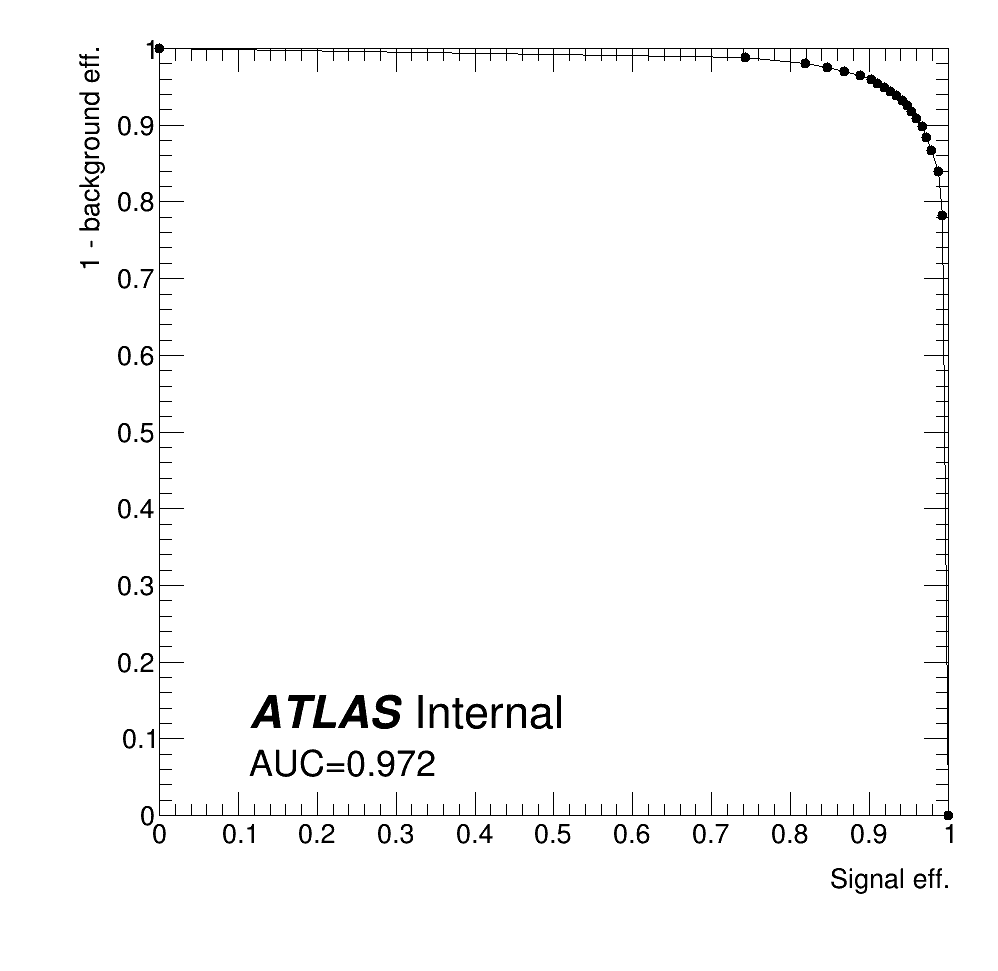
\includegraphics[width=0.45\textwidth]{images/AnalysisStrategy/ROCCurve_Hp2500_Contained80_DL1r_70.png}
        \label{fig:ROCCurve_Hp2500}
      }
      \caption{BDT distribution and ROC curve for the 2500 GeV $H^{+}$ mass hypothesis.}
      \label{fig:BDTTrainingResults_Hp2500}
    \end{figure}
    
    %--- BDT template H+(3000)
    \begin{figure}[H]
      \centering
      \subfloat[BDT output]{
        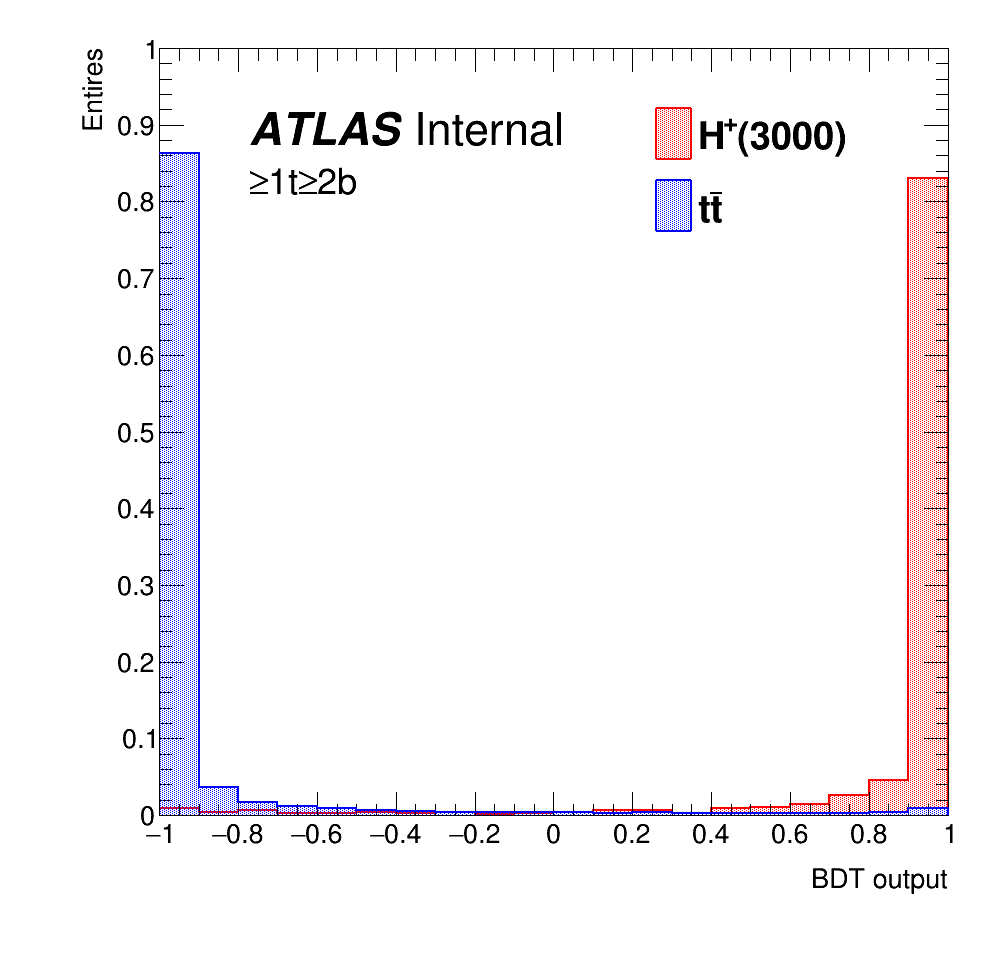
\includegraphics[width=0.45\textwidth]{images/AnalysisStrategy/BDTOutput_Hp3000_Contained80_DL1r_70.png}
        \label{fig:BDTOutput_Hp3000}
      }
      \subfloat[ROC curve]{
        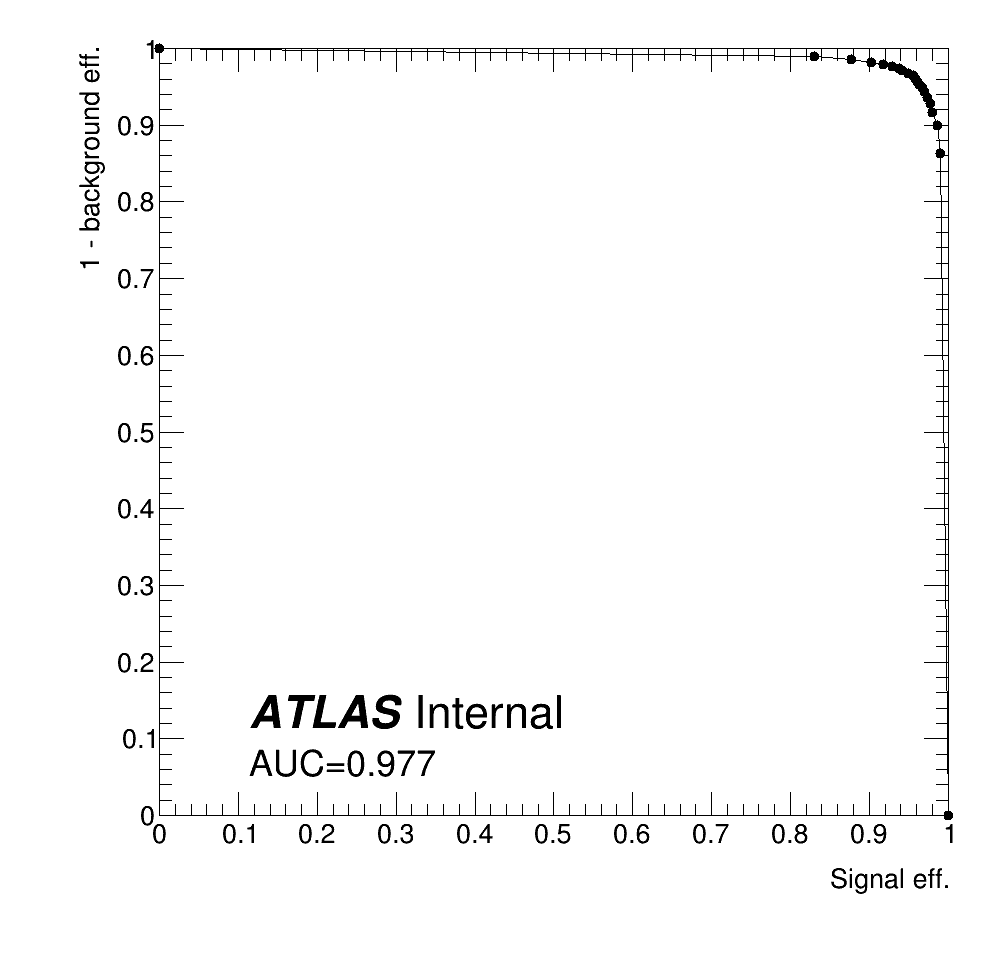
\includegraphics[width=0.45\textwidth]{images/AnalysisStrategy/ROCCurve_Hp3000_Contained80_DL1r_70.png}
        \label{fig:ROCCurve_Hp3000}
      }
      \caption{BDT distribution and ROC curve for the 3000 GeV $H^{+}$ mass hypothesis.}
      \label{fig:BDTTrainingResults_Hp3000}
    \end{figure}

    \item{\textbf{Comparison of BDT distributions between $H^{+} \rightarrow tb$ and  $W' \rightarrow tb$ events}}\mbox{}\\
    BDT distributions for $W' \rightarrow tb$ events are compared with the ones for $H^{+} \rightarrow tb$ events in Figure \ref{fig:CompHpAndWp}. The large differences above their statistic uncertainty are not observed. Therefore, it is expected to be able to obtain comparable sensitivity with $H^{+} \rightarrow tb$ analysis without further optimization using $W' \rightarrow tb$ samples.

    %--- Comparison of BDT outputs between H+ and W'
    \begin{figure}[H]
        \centering
        \subfloat[$M=1.0$ TeV]{
            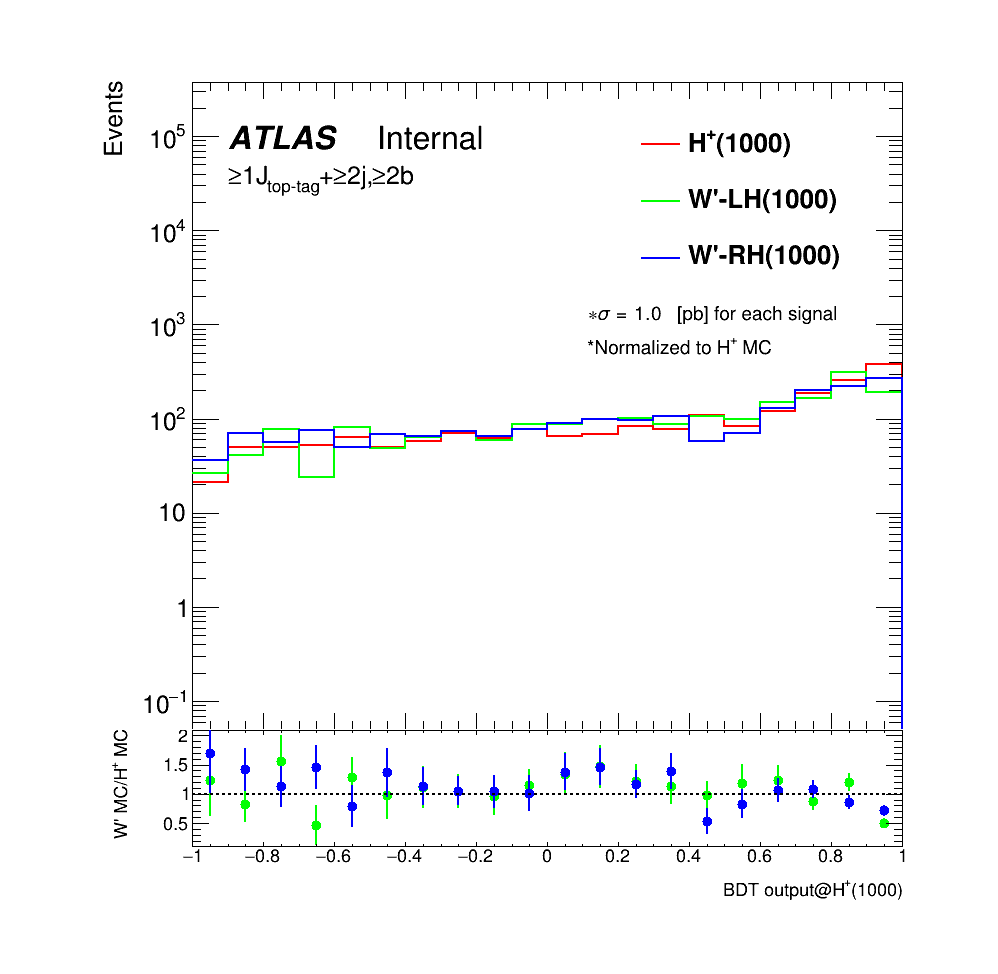
\includegraphics[width=0.45\textwidth]{images/AnalysisStrategy/bdt_Hp1000_1000_geq1tgeq2jgeq2b.png}
            \label{fig:CompHpAndWp_M1000}
        }
        \subfloat[$M=1.2$ TeV]{
            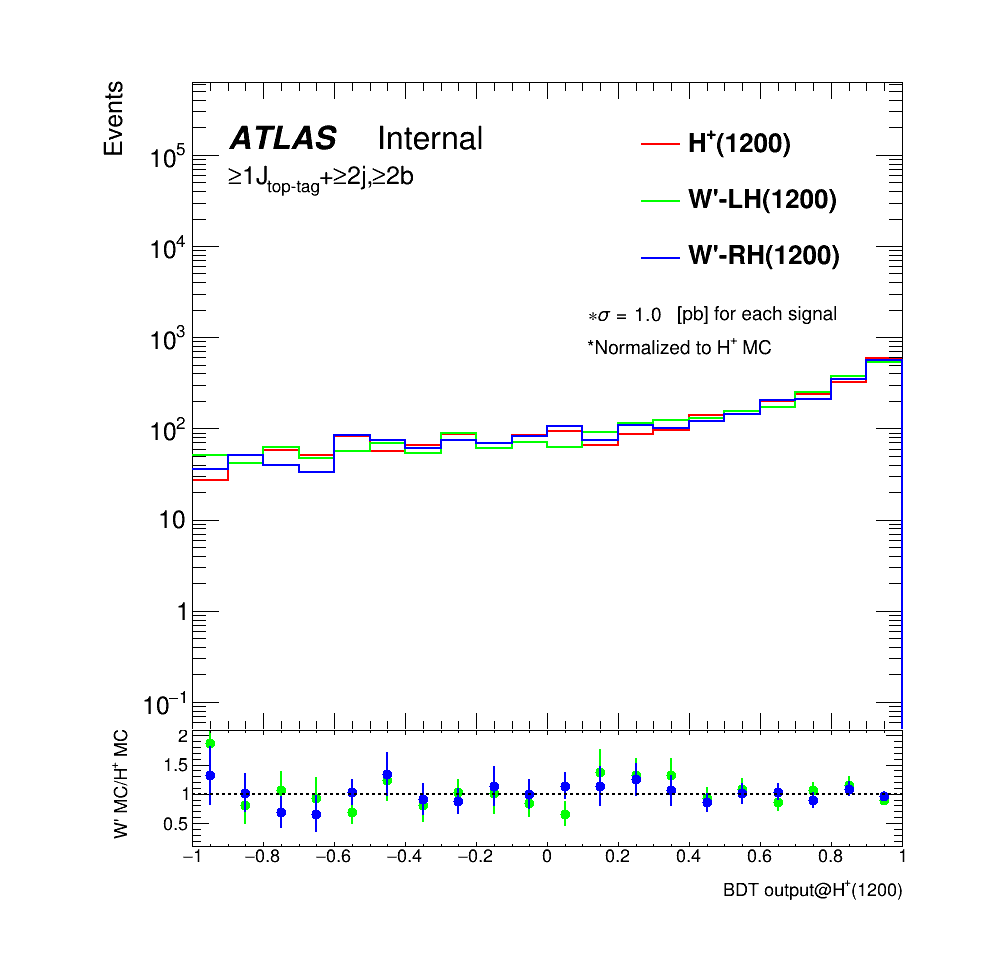
\includegraphics[width=0.45\textwidth]{images/AnalysisStrategy/bdt_Hp1200_1200_geq1tgeq2jgeq2b.png}
            \label{fig:CompHpAndWp_M1200}
        }\\
        \subfloat[$M=1.4$ TeV]{
            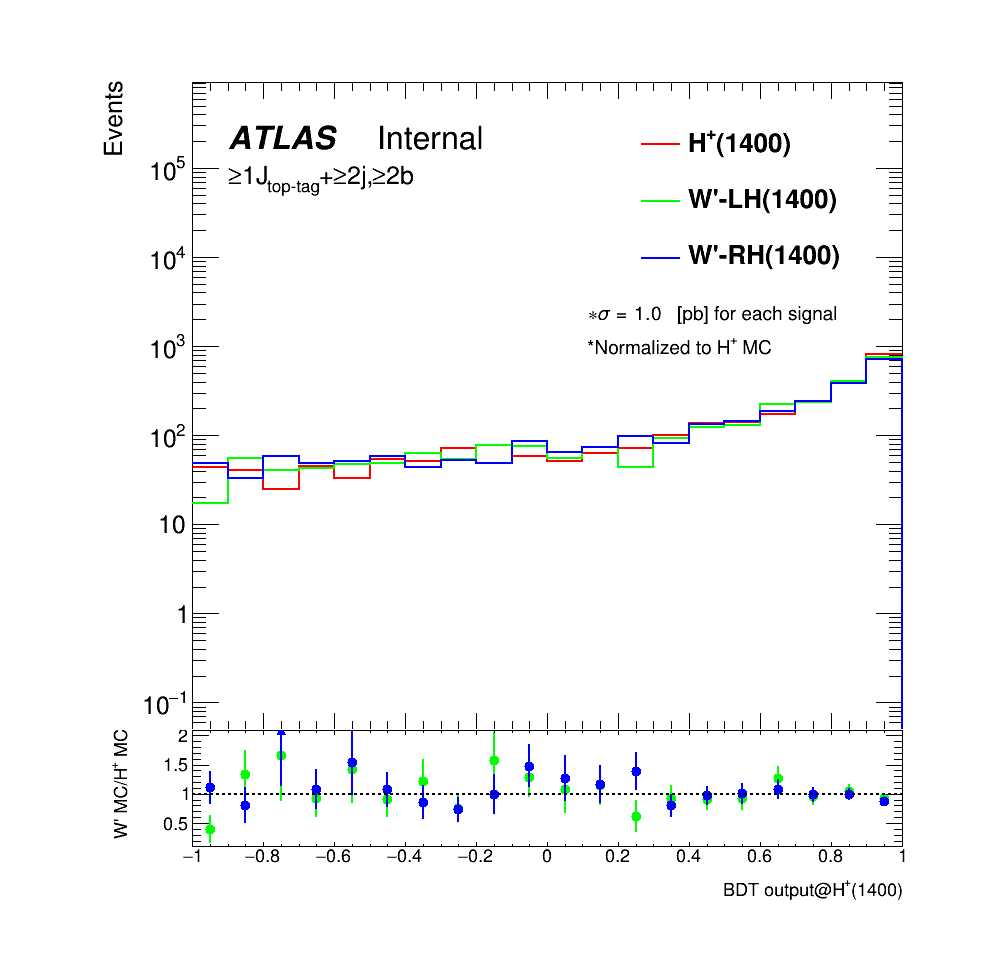
\includegraphics[width=0.45\textwidth]{images/AnalysisStrategy/bdt_Hp1400_1400_geq1tgeq2jgeq2b.png}
            \label{fig:CompHpAndWp_M1400}
        }  
        \subfloat[$M=1.6$ TeV]{
            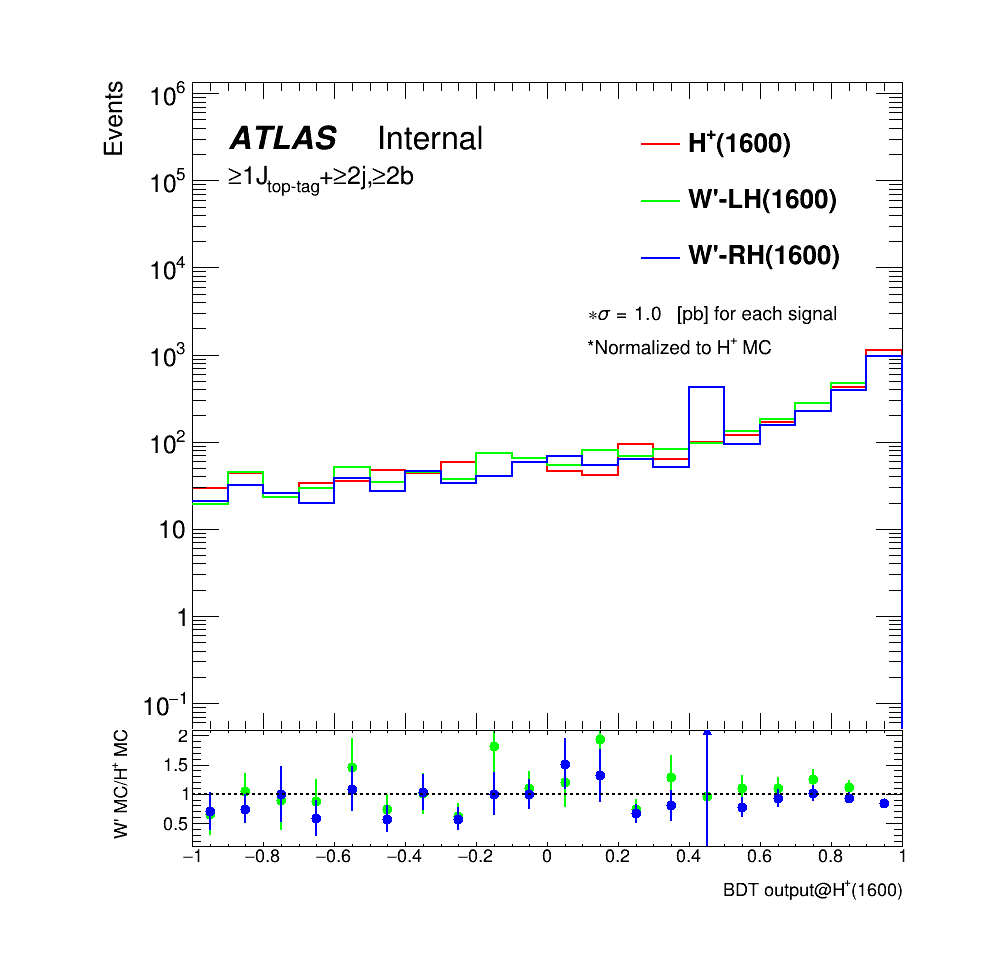
\includegraphics[width=0.45\textwidth]{images/AnalysisStrategy/bdt_Hp1600_1600_geq1tgeq2jgeq2b.png}
            \label{fig:CompHpAndWp_M1600}
        }\\
    \end{figure}
    \begin{figure}[H]
        \addtocounter{figure}{-1}
        \subfloat[$M=1.8$ TeV]{
             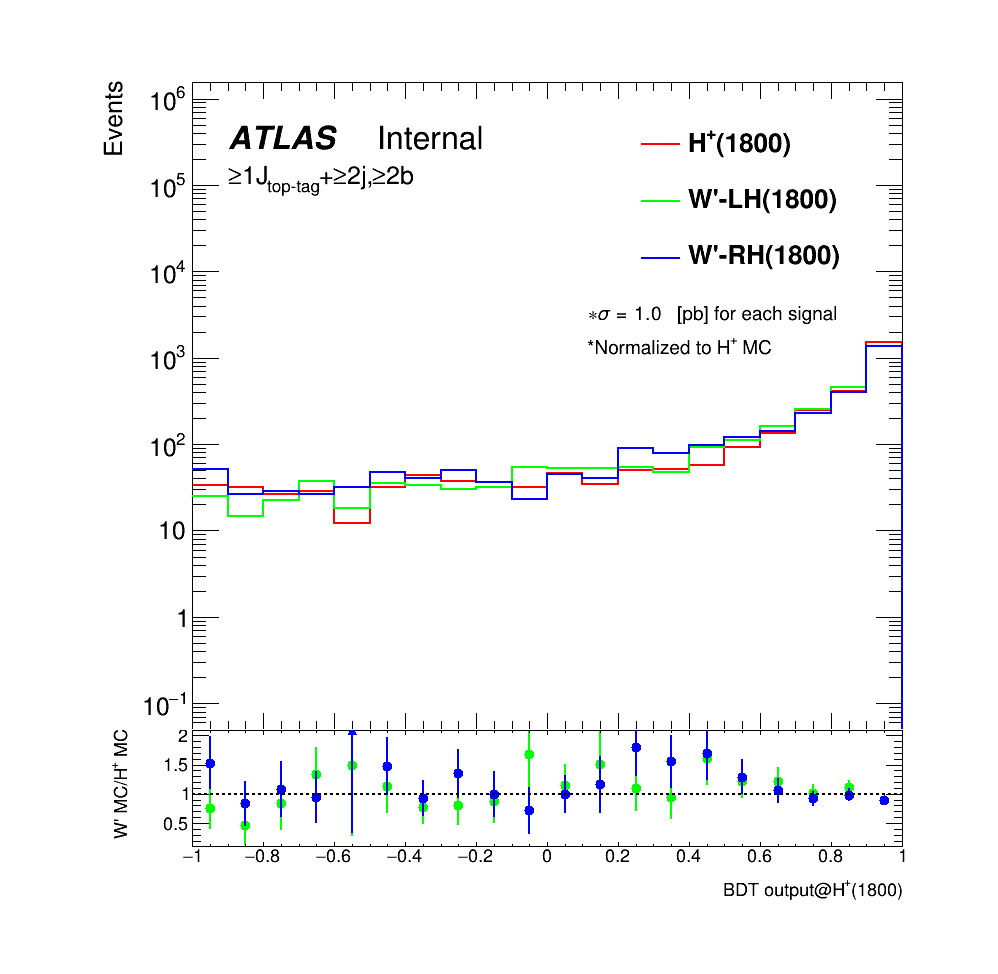
\includegraphics[width=0.45\textwidth]{images/AnalysisStrategy/bdt_Hp1800_1800_geq1tgeq2jgeq2b.png}
             \label{fig:CompHpAndWp_M1800}
        }
        \subfloat[$M=2.0$ TeV]{
            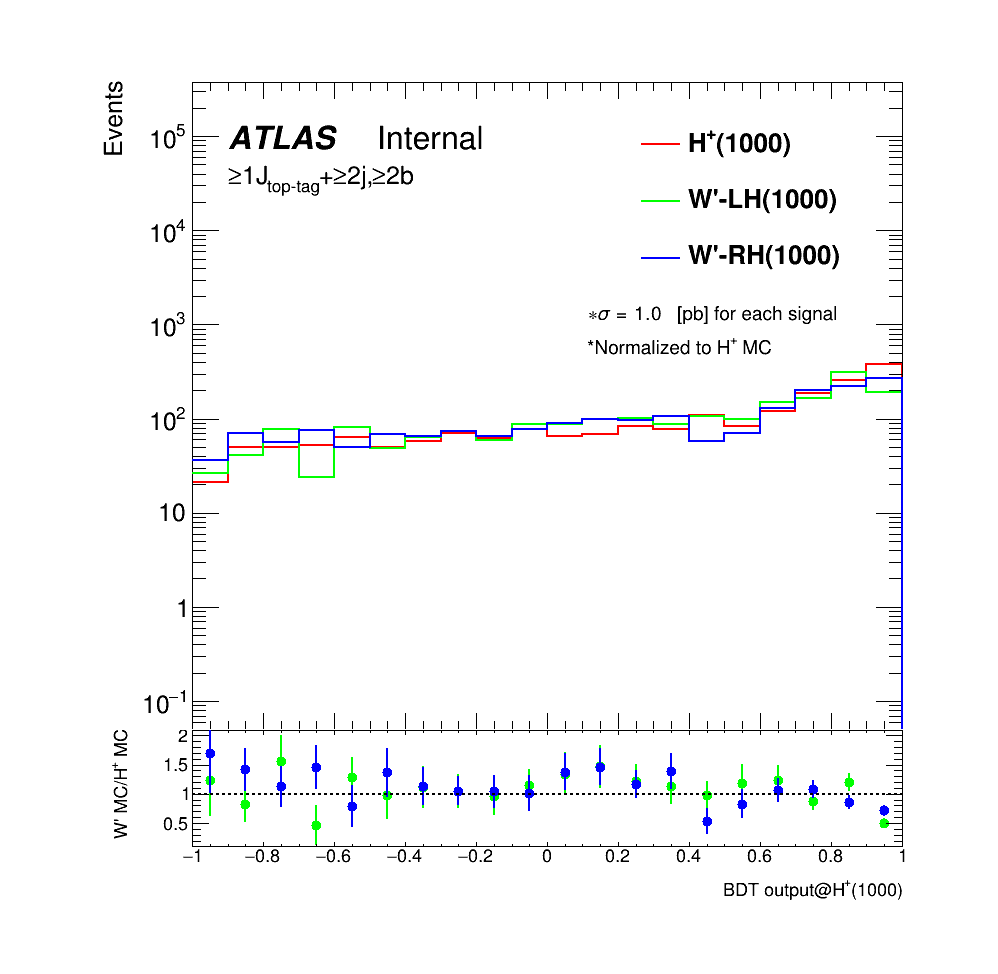
\includegraphics[width=0.45\textwidth]{images/AnalysisStrategy/bdt_Hp1000_1000_geq1tgeq2jgeq2b.png}
            \label{fig:CompHpAndWp_M2000}
        }\\
        \subfloat[$M=2.5$ TeV]{
            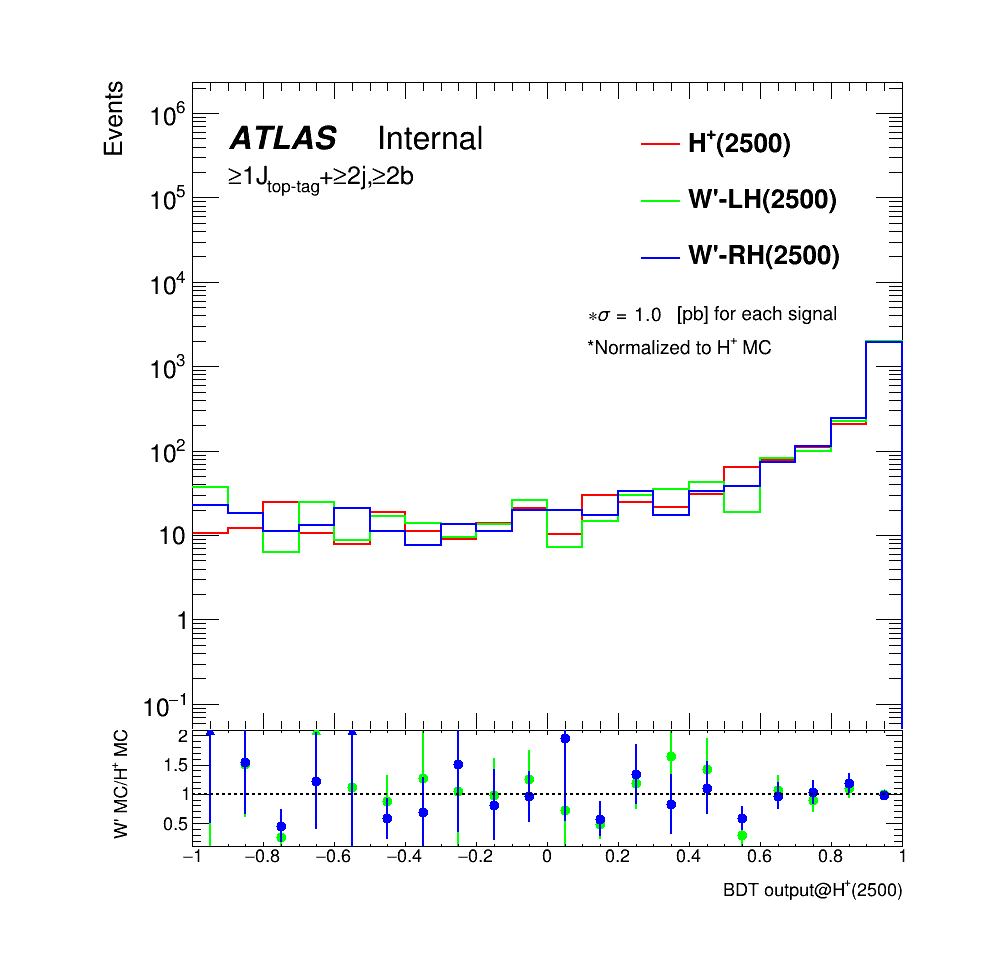
\includegraphics[width=0.45\textwidth]{images/AnalysisStrategy/bdt_Hp2500_2500_geq1tgeq2jgeq2b.png}
            \label{fig:CompHpAndWp_M2500}
        }  
        \subfloat[$M=3.0$ TeV]{
            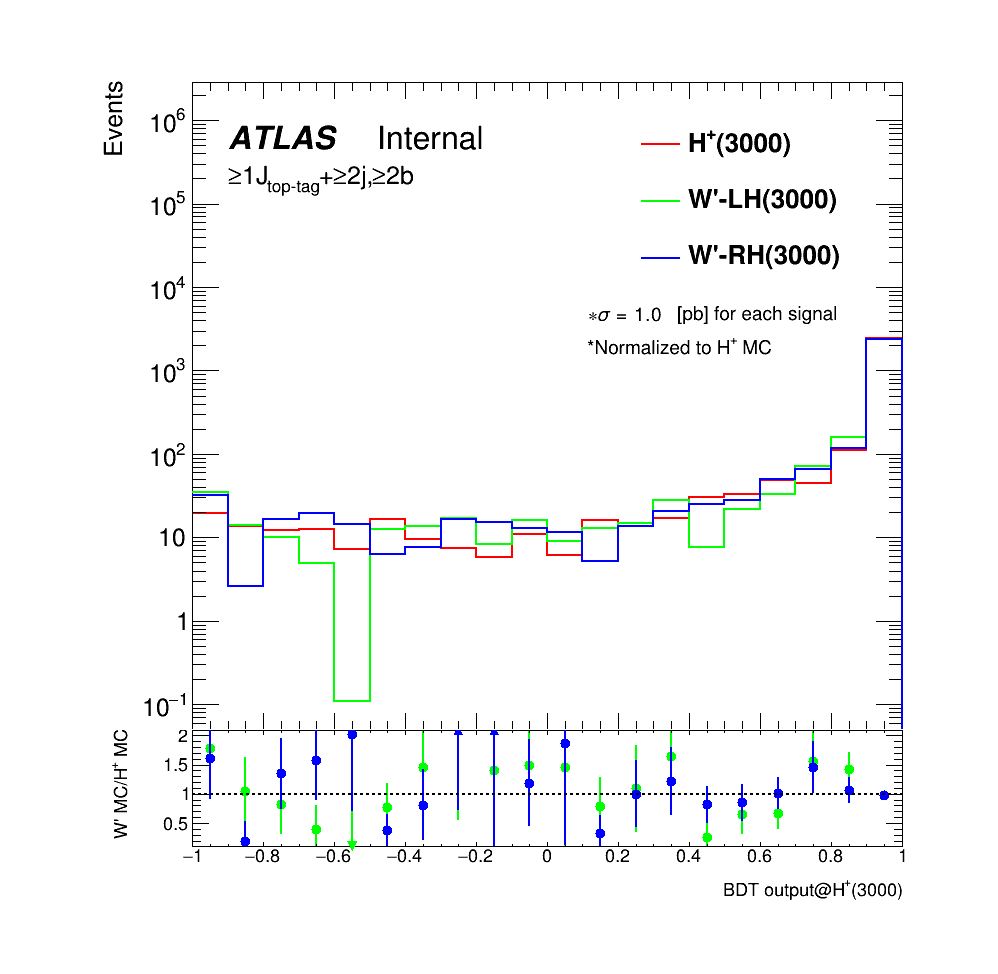
\includegraphics[width=0.45\textwidth]{images/AnalysisStrategy/bdt_Hp3000_3000_geq1tgeq2jgeq2b.png}
            \label{fig:CompHpAndWp_M3000}
        }
        \caption{Comparison of BDT distributions between $H^{+} \rightarrow tb$ and  $W' \rightarrow tb$ events in the inclusive SR (i.e., SR1+SR2).}
        \label{fig:CompHpAndWp}
    \end{figure}
    
\end{description}

\subsection{Analysis strategy above 3 TeV}
\label{subsec:AnaStrategyAbove3TeV}
For the mass point above 3 TeV, we adopt a different approach. Since it is difficult to estimate $t\bar{t}+\text{jets}$ events reliably in the very high $H_{\text{T}}^{\text{jets}}$ region where most of the signal events distribute, we use a cut-and-counting method as detailed below, which avoids using the line shapes at the high $H_{\text{T}}^{\text{jets}}$ region, and therefore is more robust against potential mis-modelling compared with the BDT method. 

\begin{figure}[H]
    \subfloat[]{
        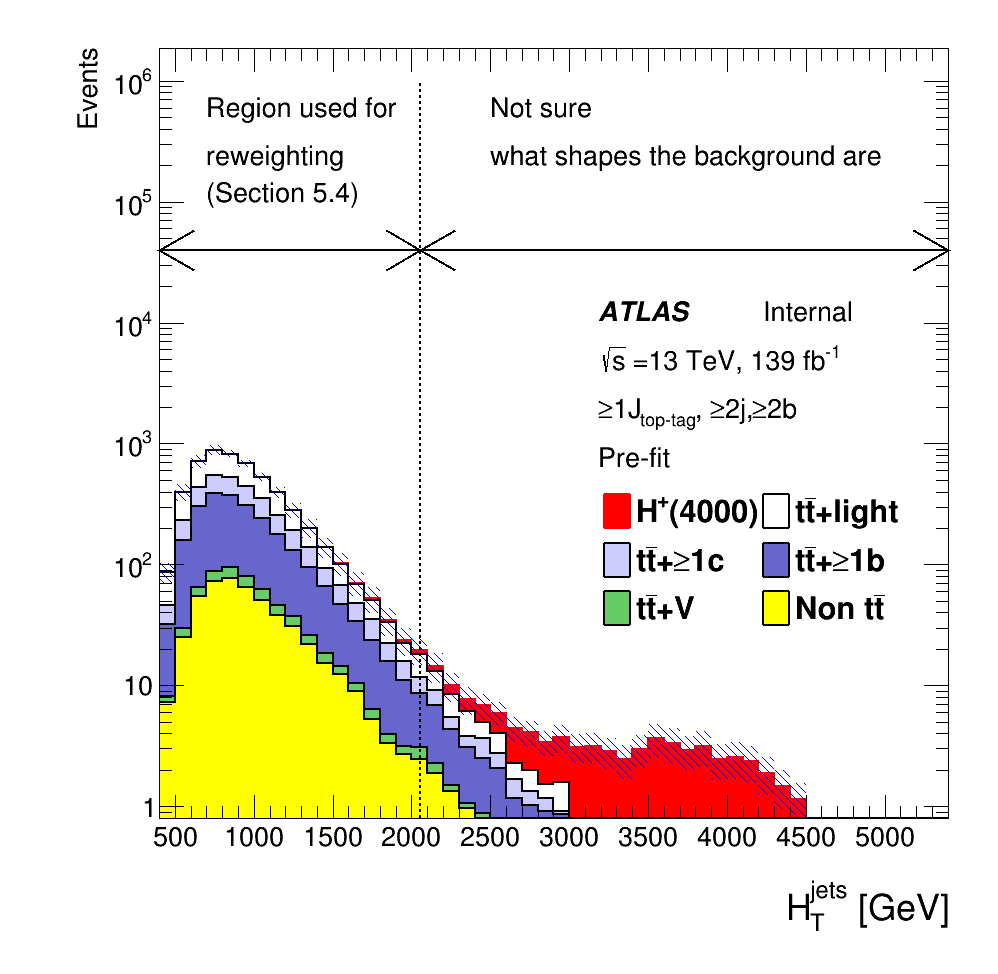
\includegraphics[width=0.45\textwidth]{images/AnalysisStrategy/SOVERB_Hp4000_Contained80_DL1r_70_HTjets_beforeRW_geq1tgeq2jgeq2b_prefit.png}
        \label{fig:SOVERB_HT_jets_4000GeV}
    }
    \subfloat[]{
        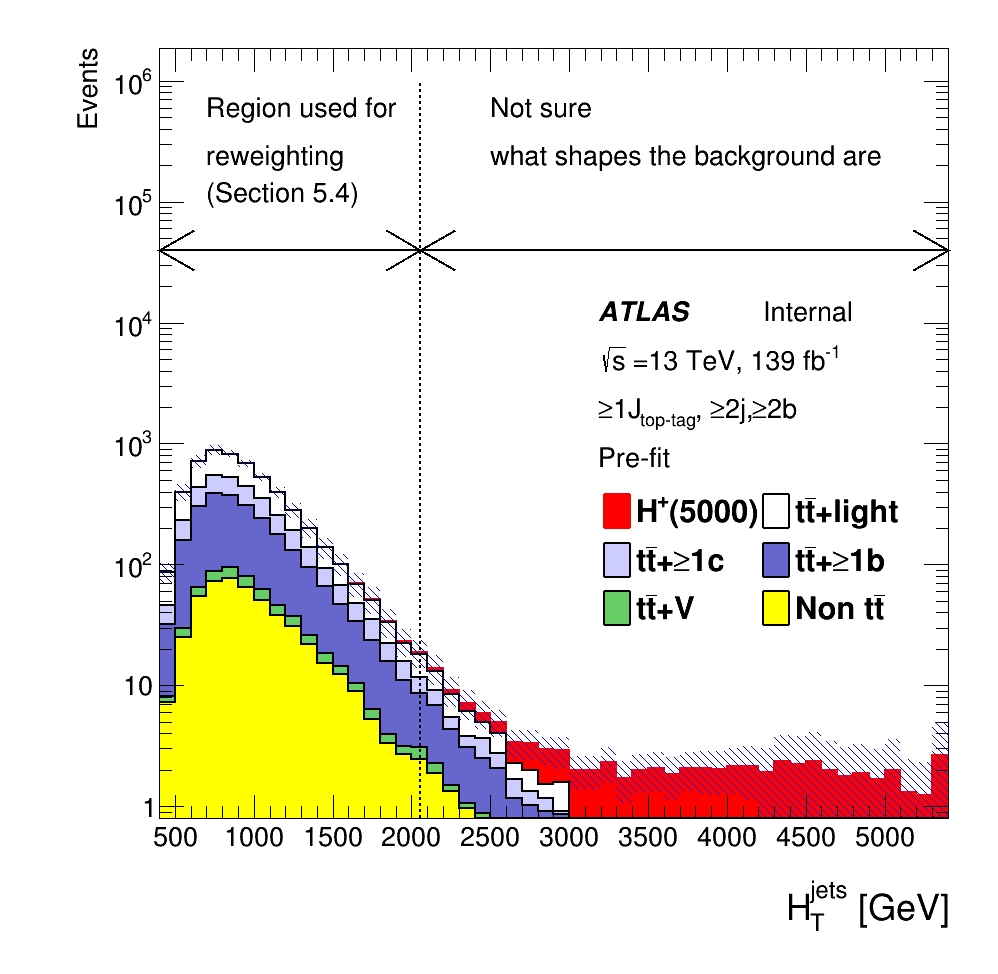
\includegraphics[width=0.45\textwidth]{images/AnalysisStrategy/SOVERB_Hp5000_Contained80_DL1r_70_HTjets_beforeRW_geq1tgeq2jgeq2b_prefit.png}
        \label{fig:SOVERB_HT_jets_5000GeV}
    }
    \caption{Signal and background comparison for 4000 (a) and 5000 (b) GeV mass hypotheses. These signal events distribute mostly in $H_{\text{T}}^{\text{jets}}>2000$ GeV. These regions don't have enough shape information to perform reweighting in Section \ref{subsec:ReweightingTechnique}.}
    \label{fig:SOVERB_HT_jets_4and5TeV}
\end{figure}

One signal region (SR) and two control regions (CR1, CR2) are defined according to the $H_{\text{T}}^{\text{jets}}$ and the number of $b$-jets. All events are first required to satisfy the same selection criteria for the inclusive SR of the multivariate analysis (discussed in Section \ref{subsubsec:RegionDefUnder3TeV}). They are categorized in the SR if they have $H_{\text{T}}^{\text{jets}}>2000$ GeV, while events with $H_{\text{T}}^{\text{jets}} \leq 2000$ are categorized into the CR1 and CR2, depending on $\text{N}_{b_{\text{jets}}}$. For CR1 (CR2), $\text{N}_{b-\text{jets}}=2 (\geq 3)$ are imposed. After these selections, the CR1 becomes enriched in $t\bar{t}+\text{light}$ events, while the CR2 becomes enriched in $t\bar{t}+\text{HF}$, similarly to SR1 and SR2, respectively, of the multivariate analysis. The event selections in these regions are summarized in Table \ref{tab:EventSelectionInSRAndCR1AndCR2}. $H_{\text{T}}^{\text{jets}}$ is used as final discriminates, as discussed in Section \ref{sec:ProfileLikelohoodFit}. The number of bins of $H_{\text{T}}^{\text{jets}}$ distribution in the SR is set to one. These distributions and the composition ratio of backgrounds for these regions are shown in Figure \ref{fig:BkgComposition_SR} to Figure \ref{fig:BkgComposition_CR2}. 

\begin{table}[H]
    \centering
    \begin{tabular*}{130mm}{c|c|c|c}
        \hline\hline
        Cut                          & SR & CR1 & CR2\\
        \hline
        leptons                      & \multicolumn{3}{c}{Same requirements as Table \ref{tab:EventSelectionInSR1AndSR2}}\\
        \hline
        Top-tagged large-$R$ jets    & \multicolumn{3}{c}{Same requirements as Table \ref{tab:EventSelectionInSR1AndSR2}}\\
        \hline
        Small-$R$ jets               & \multicolumn{2}{c|}{$\text{N}_{\text{jet}} \geq 2$}  & $\text{N}_{\text{jet}} \geq 3$ \\
                                     & \multicolumn{2}{c|}{(Kinematic requirements}  & (Kinematic requirements \\
                                     & \multicolumn{2}{c|}{are the same as Table \ref{tab:EventSelectionInSR1AndSR2})} & are the same as Table \ref{tab:EventSelectionInSR1AndSR2})\\
        \hline
        $b$-tagged small-$R$ jets    & $\text{N}_{b-\text{jet}} \geq 2$ & $\text{N}_{b-\text{jet}} = 2$  & $\text{N}_{b-\text{jet}} \geq 3$\\
        \hline
        $H_{\text{T}}^{\text{jets}}$ & $> 2000$ GeV & \multicolumn{2}{c}{$\leq 2000$ GeV}\\
        \hline\hline
  \end{tabular*}
  \caption{Event selections in the SR, CR1, and CR2. After these selections, CR1 becomes enriched in $t\bar{t}+\text{light}$, and CR2 becomes enriched in $t\bar{t}+\text{HF}$.}
  \label{tab:EventSelectionInSRAndCR1AndCR2}
\end{table}

%--- Figure for SR
\begin{figure}[H]
  \centering
  \subfloat[]{
    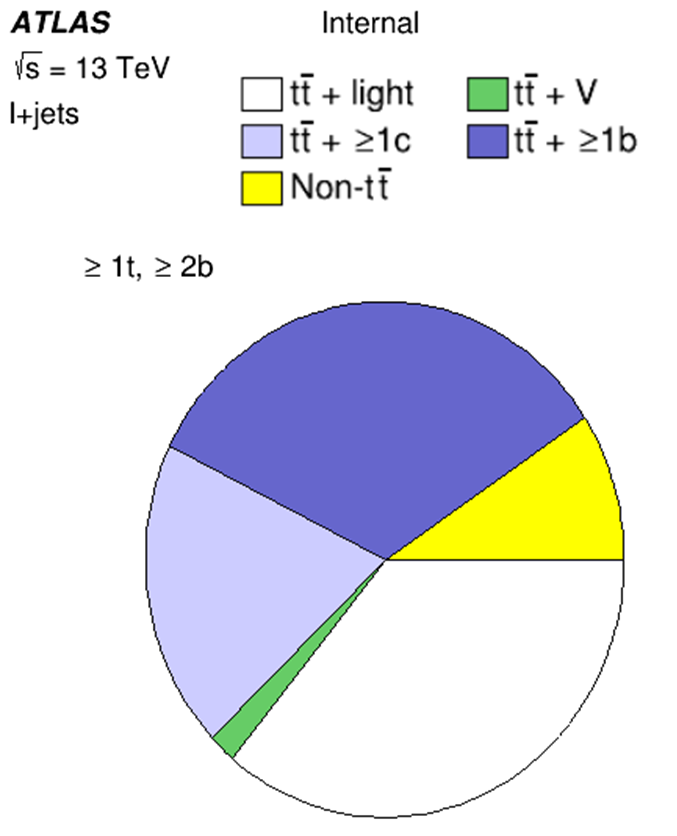
\includegraphics[keepaspectratio,scale=0.2]{images/AnalysisStrategy/PieChart_SR.png}
    \label{fig:PieChart_SR}
  }
  \subfloat[]{
    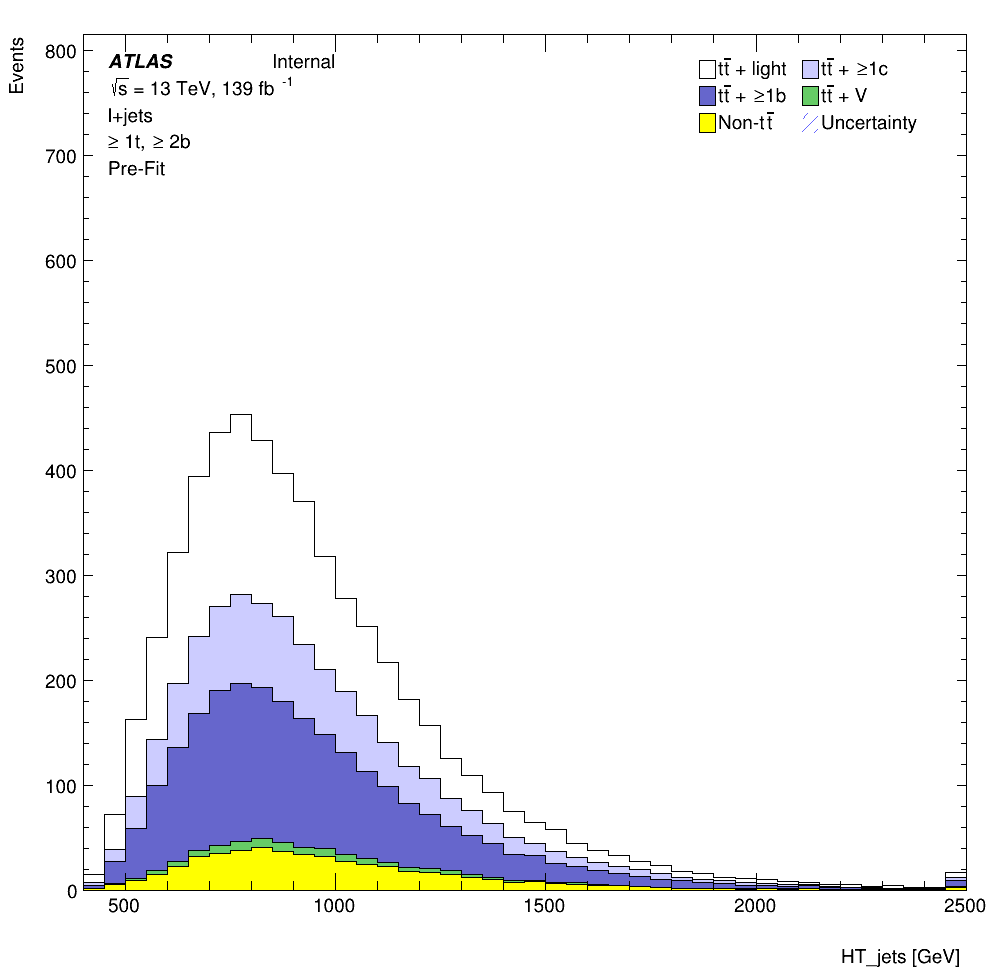
\includegraphics[keepaspectratio,scale=0.2]{images/AnalysisStrategy/HT_jets_SR.png}
    \label{fig:PieChart_SR1}
  }
  \caption{Background composition in the SR is shown in the pie chart (a) and the $H_{\text{T}}^{\text{jets}}$ distributions (b). The number of bins of $H_{\text{T}}^{\text{jets}}$ distribution is set to exactly one.}
  \label{fig:BkgComposition_SR}
\end{figure}

%--- Figure for CR1
\begin{figure}[H]
  \centering
  \subfloat[]{
    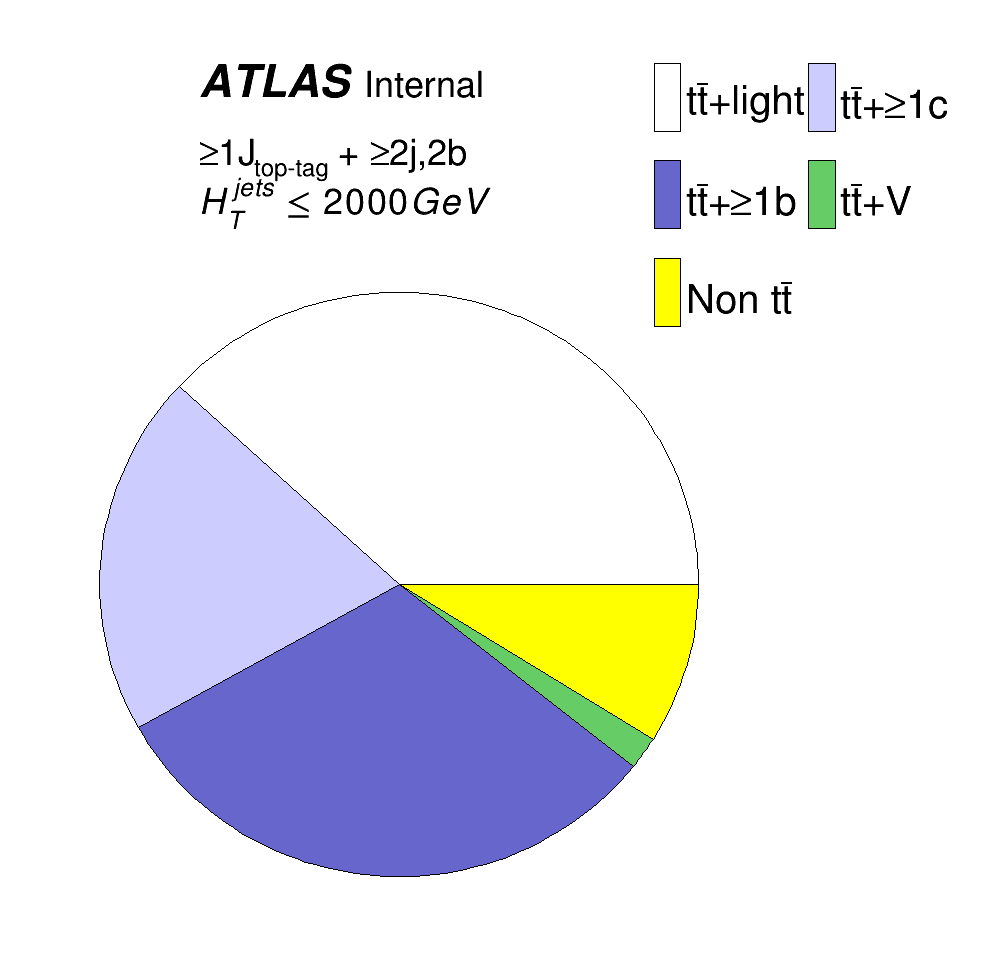
\includegraphics[keepaspectratio,scale=0.2]{images/AnalysisStrategy/PieChart_CR1.png}
    \label{fig:PieChart_CR1}
  }
  \subfloat[]{
    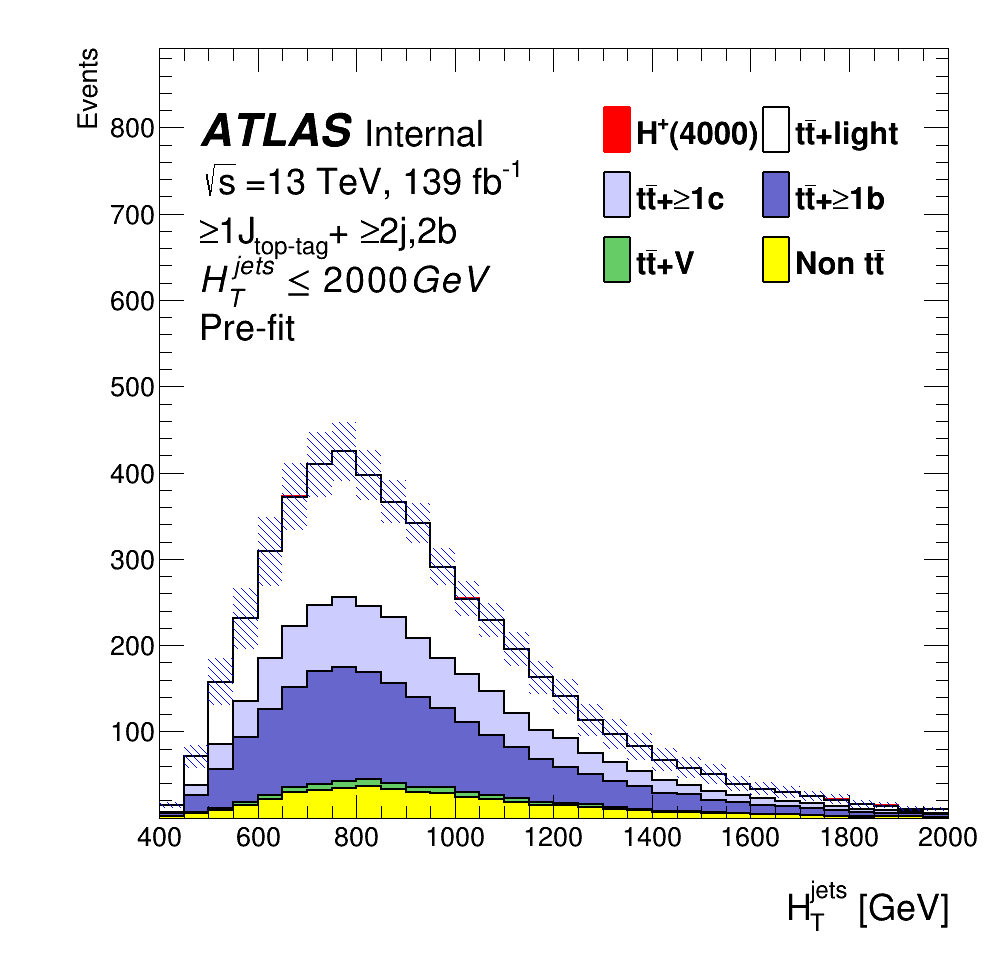
\includegraphics[keepaspectratio,scale=0.2]{images/AnalysisStrategy/HT_jets_CR1.png}
    \label{fig:PieChart_CR1}
  }
  \caption{Background composition in the CR1 is shown in the pie chart (a) and the $H_{\text{T}}^{\text{jets}}$ distributions (b).}
  \label{fig:BkgComposition_CR1}
\end{figure}

%--- Figure for CR1
\begin{figure}[H]
  \centering
  \subfloat[]{
    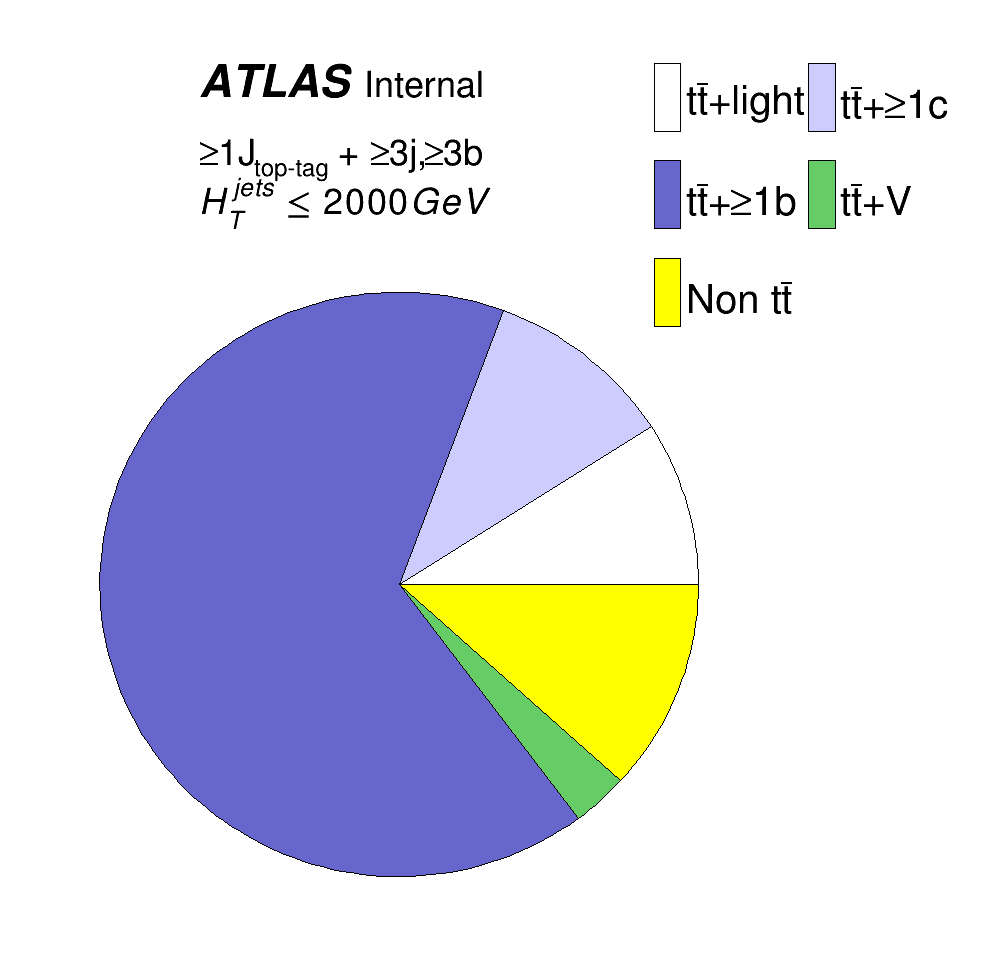
\includegraphics[keepaspectratio,scale=0.2]{images/AnalysisStrategy/PieChart_CR2.png}
    \label{fig:PieChart_CR2}
  }
  \subfloat[]{
    \includegraphics[keepaspectratio,scale=0.2]{images/AnalysisStrategy/HT_jets_CR2.png}
    \label{fig:PieChart_CR2}
  }
  \caption{Background composition in the CR2 is shown in the pie chart (a) and the $H_{\text{T}}^{\text{jets}}$ distributions (b).}
  \label{fig:BkgComposition_CR2}
\end{figure}

The number of expected signal and background events in the SR, CR1, and CR2 are shown in Table \ref{tab:PrefitYieldsAbove3TeV}. The predicted number of $H^{+}$ and $W'$ signal events for the 4000 and 5000 GeV mass hypothesis are estimated using $\sigma \times Br = 0.046$ pb, as done in Table \ref{tab:PrefitYields}.

\begin{table}[H]
  \centering
  \begin{tabular*}{130mm}{@{\extracolsep{\fill}}cccc}
    \hline\hline
                            & SR           & CR1             & CR2\\
    \hline
    $t\bar{t}+\text{light}$ & $21 \pm  3$  & $1920 \pm 162$  & $ 34 \pm  5$\\
    $t\bar{t}+\geq1c$       & $11 \pm  9$  & $1007 \pm 782$  & $ 39 \pm 37$\\
    $t\bar{t}+\geq1b$       & $21 \pm 10$  & $1568 \pm 794$  & $249 \pm 46$\\
    $t\bar{t}+W$            & $ 1 \pm  0$  & $  35 \pm   6$  & $  2 \pm  0$\\
    $t\bar{t}+Z$            & $ 1 \pm  0$  & $  57 \pm   8$  & $  9 \pm  2$\\
    $Wt$ channel            & $ 3 \pm  3$  & $ 173 \pm 101$  & $  7 \pm  4$\\
    $t$ channel             & $ 1 \pm  0$  & $  35 \pm  16$  & $ 16 \pm  1$\\
    Other top sources       & $ 1 \pm  0$  & $  28 \pm  12$  & $  8 \pm  4$\\
    $VV$, $V$+jets          & $ 5 \pm  2$  & $ 132 \pm  53$  & $  4 \pm  2$\\
    $t\bar{t}H$             & $ 1 \pm  0$  & $  78 \pm   3$  & $ 24 \pm  1$\\
    \hline
    Total                   & $65 \pm  7$  & $5033 \pm 308$  & $377 \pm 33$\\
    \hline
    $H^{+}$ 4000 GeV        & $57 \pm 18$  & $   5 \pm   2$  & $  2 \pm  0$\\
    $H^{+}$ 5000 GeV        & $55 \pm 27$  & $   3 \pm   1$  & $  1 \pm  0$\\
    \hline\hline
  \end{tabular*}
  \caption{Number of expected and selected events split according to the SR, CR1, and CR2. The quoted uncertainties include both statistical and systematic uncertainties before fitting.}
  \label{tab:PrefitYieldsAbove3TeV}
\end{table}